%----------------------------------------------------------------------------------------
%	The Perceptron CHAPTER 
%----------------------------------------------------------------------------------------
\chapterimage{ChapterCover.pdf} % Chapter heading image
\chapter{Typesetting with \LaTeX{}}

\epigraph{\textit{Style means the right word. The rest matters little.}}{\rightline{{\rm --- \href{https://en.wikipedia.org/wiki/Jules_Renard}{Jules Renard}}}}

\minitoc
\newpage
\section{What is \LaTeX{} ?}
\LaTeX{}, pronounced ``Lay-tech'' or ``Lah-tech'', is a high quality typesetting system; it includes features designed for the production of technical and scientific documentation. \LaTeX{} is widely used in academia for the communication and publication of scientific documents in many fields, including mathematics, statistics, quantitative psychology, computer science, engineering, chemistry, physics, economics, linguistics, philosophy, and political science. It also has a prominent role in the preparation and publication of books and articles that contain complex elements. \LaTeX{} is available for free at \weblink{https://www.latex-project.org/}.

When using \LaTeX{}, the writer uses plain text as opposed to the formatted text found in WYSIWYG (``what you see is what you get'') word processors like Microsoft Word, Google Docs, LibreOffice Writer and Apple Pages. In LaTeX, the writer uses markup tagging conventions to define the general structure of a document (such as article, book, and letter), to stylize text throughout a document (such as bold and italics), and to add citations and cross-references.

To make clear how \LaTeX{} is different from WYSIWYG word-processing software you are likely already familiar with, consider that In most publishing environments, the author first submits his or her text for publication.  Next, a human designer determines what the layout of the publication will be (i.e., headers, headings, images, etc.).  Finally, a typesetter combines the author’s text and instructions from the designer to create the finished product.  In this example, LaTeX takes on the role of designer and TeX the role of typesetter.  This is quite different from the WYSIWYG approach that most modern word processors, such as MS Word or LibreOffice, take. With these applications, authors specify the document layout interactively while typing text into the computer. They can see on the screen how the final work will look when it is printed, taking on the roles of author, designer, and typesetter.


\subsection*{Why \LaTeX{} ?}
The first question asked by most WYSIWYG users upon hearing a description of \LaTeX{} is, Why?   It is my humble opinion that using LaTeX is a bit like bringing a calculator to a math test. If you know how to use it, it can make things so much easier - so much easier it feels like cheating. When you know how to use LaTeX, you won’t have to remember anything about APA formatting. LaTeX will take care of everything for you. All you have to do is focus on your writing.  Still, it is common for WYSIWYG and LaTeX users to debate about the pros and cons of each approach.  Thus, a few of the most commonly promoted advantages and disadvantages of using LaTeX are listed below.

\vspace{.2cm}
\noindent \begin{tabularx}{\textwidth}{@{}X X@{}}
\textbf{Advantages} &
\textbf{Disadvantages} \\ \\
\begin{itemize}[leftmargin=*]
  \item \LaTeX{} frees the author to focus almost entirely on content
  \item Many layouts are available, producing professionally crafted documents
  \item Output is consistent and replicable
  \item Excellent typesetting of mathematical formulae
  \item Easy generation of complex structures (footnotes, references, TOC, bibliographies)
  \item User-friendly over time: once you learn the basics, it's easy to get help online
  \item Most LaTeX editors have a user-friendly interface
  \item Rich documentation due to long history
  \item High-quality illustrations with PSTricks or TikZ
  \item Better at preparing complex tables
\end{itemize}
&
\begin{itemize}[leftmargin=*]
  \item Fairly steep learning curve
  \item Collaborators unfamiliar with \LaTeX{} may have difficulty reviewing your manuscripts
  \item Many features require additional libraries (e.g., to track changes)
  \item Custom layout changes can be time-consuming to implement
  \item No native spell-check or grammar-check
\end{itemize}
\end{tabularx}

\subsection*{Getting \LaTeX{}}
LaTeX is free software under the terms of the LaTeX Project Public License (LPPL). LaTeX is distributed through CTAN servers or comes as part of many easily installable and usable TeX distributions provided by the TeX User Group (TUG) or third parties.  Below are the recommended distributions for the most popular operating systems.

\vspace{.2cm}
\rowcolors{2}{gray!5}{gray!10} % Optional row striping
\begin{tabularx}{\textwidth}{>{\raggedright\arraybackslash}p{3cm} X}
\rowcolor{gray!40}
\textbf{Platform} & \textbf{Instructions} \\

Linux &
Installing the \texttt{TeX Live} distribution is advisable, as many Linux distributions only contain older versions. See the official TeX Live documentation for package status and installation details. \\

Mac OS &
The \texttt{MacTeX} distribution contains everything you need, including a complete TeX system with \LaTeX{} itself and user-friendly editors to write documents. \\

Windows &
Check out the \texttt{MiKTeX}, \texttt{proTeXt}, or \texttt{TeX Live} distributions. They all contain a complete TeX system with \LaTeX{} and editors for writing documents. \\

Online (cloud-based) &
\LaTeX{} online services like \texttt{Overleaf}, \texttt{Papeeria}, \texttt{Datazar}, and \texttt{LaTeX Base} let you edit, view, and download \LaTeX{} files and resulting PDFs in your browser. These are great for beginners or collaboration. \\
\end{tabularx}

\subsection*{Using \LaTeX{}}

Once you have started a new blank document, or decided on a template, it’s time to start editing. Once you open a project, the screen will be divided into three sections.  On the far left, you will find a view of the current working directory for the project where you will see all of the files associated with the current project and find options for upload files (e.g., figures and images). The middle section is the editor where you will write and make changes to the content of your document. Finally, the right section is the output viewer, which allows you to preview your document after being compiled with TeX formatting, but without having to save it as a PDF. By default it is set to automatically update as changes are made, but it can be toggled to a manual option.  The project screens in Overleaf and the TexMaker IDE (just for comparison) are illustrated below.

\begin{center}
\myfigure{Common \LaTeX{} Editors}{Introduction2LaTeX/figures/latexeditors.PNG}{Most editors have three panels: (1) A file directory, (2) an editor, and (3) an ouput viewer.}{fig:latexeditors}{.9\linewidth}{\linewidth}{\linewidth}
\end{center}

When editing a project there are two options to select from in Overleaf: Source and Rich Text. Both can use the toolbar that inserts code for you for particular actions, but will look different in their set-up. The Rich Text option creates a WYSIWYG type interface where formatting is mostly done by clicking buttons rather than coding by hand. This can be useful when getting familiar with \LaTeX{}, but this tutorial will focus primarily on Source editing.

\section{\LaTeX{} Preliminaries}
Before you start adding content to your document, there are a few important things to know about the LaTeX environment.

\subsection*{Spaces}
``Whitespace'' characters, such as blank or tab, are treated uniformly as ``space'' by LATEX. Several consecutive whitespace characters are treated as one ``space''. Whitespace at the start of a line is generally ignored, and a single line break is treated as ``whitespace''. An empty line between two lines of text defines the end of a paragraph. Several empty lines are treated the same as one empty line. The text below is an example. On the left hand side is the text from the input file, and on the right hand side is the formatted output.

\vspace{.2cm}
\noindent \begin{tabularx}{\textwidth}{@{}X X@{}}
\rowcolor{gray!40}
\multicolumn{1}{c}{\textbf{\LaTeX{}}} & 
\multicolumn{1}{c}{\textbf{Formatted Output}} \\
\texttt{It}\hspace{.3cm}\texttt{ does not matter}\hspace{.4cm} \texttt{whether you} \hspace{.3cm}  \texttt{enter one or several } \hspace{.5cm} \texttt{ spaces after a} \hspace{.5cm} \texttt{ word.} 

\texttt{An empty line starts a new paragraph.}
&
It does not matter whether you enter one or several spaces after a word. 

An empty line starts a new paragraph.
\end{tabularx}


\subsection*{Comments}
When \LaTeX{} encounters a \% character while processing an input file, it ignores the rest of the line, the line break, and all whitespace at the beginning of the next line. This can be used to write notes into your document that will not show up in the printed version.

\vspace{.2cm}
\noindent \begin{tabularx}{\textwidth}{@{}X X@{}}
\rowcolor{gray!40}
\multicolumn{1}{c}{\textbf{\LaTeX{}}} & 
\multicolumn{1}{c}{\textbf{Formatted Output}} \\
\texttt{This is a \%stupid \newline
great example of using the \% character to add comments to a document.}
&
This is a great example of using the \% character to add comments to a document.
\end{tabularx}

\subsection*{Special Characters}
There are a number of special characters\/symbols that are reserved characters that either have a special meaning in \LaTeX{} or are not available in all the fonts. If you enter them directly in your text, they will normally not print, but rather coerce \LaTeX{} to do things you did not intend or potentially cause errors when compiling your document.  Some of those characters, the \LaTeX{} command required to produce them in your formatted output, and a brief description are shown below:

\vspace{.2cm}
\noindent
\begin{tabularx}{\textwidth}{@{}X X X X@{}}
\rowcolor{gray!40}
\multicolumn{1}{c}{\textbf{Symbol}} &
\multicolumn{1}{c}{\textbf{\LaTeX{}}} & 
\multicolumn{1}{c}{\textbf{Description}} & 
\multicolumn{1}{c}{\textbf{Use}} \\

\multicolumn{1}{c}{\%} &
\multicolumn{1}{c}{\texttt{\textbackslash \%}} &
\multicolumn{1}{c}{Percent} &
The comment command \\

\multicolumn{1}{c}{\$} &
\multicolumn{1}{c}{\texttt{\textbackslash \$}} &
\multicolumn{1}{c}{Dollar sign} &
Used for inline math environments \\

\multicolumn{1}{c}{\{ or \}} &
\multicolumn{1}{c}{\texttt{\textbackslash \{ }} &
\multicolumn{1}{c}{Curly braces} &
Used to create groups \\

\multicolumn{1}{c}{\#} &
\multicolumn{1}{c}{\texttt{\textbackslash \#}} &
\multicolumn{1}{c}{Number sign} &
Define function parameters in macros \\

\multicolumn{1}{c}{\&} &
\multicolumn{1}{c}{\texttt{\textbackslash \&}} &
\multicolumn{1}{c}{Amperstand} &
Separate columns in tabular environments \\

\multicolumn{1}{c}{\textbackslash} &
\multicolumn{1}{c}{\texttt{\textbackslash{}textbackslash}} &
\multicolumn{1}{c}{Backslash} &
Used to call macros \\

\multicolumn{1}{c}{\_} &
\multicolumn{1}{c}{\texttt{\textbackslash \_}} &
\multicolumn{1}{c}{Underscore} &
Indicates underscore in math mode \\

\multicolumn{1}{c}{\^{} or \~{}} &
\multicolumn{1}{c}{\texttt{\textbackslash \^{} or \textbackslash \~{}}} &
\multicolumn{1}{c}{Caret or tilde} &
Used for accents (in math) or non-breaking space (text). \\

\end{tabularx}

Note that the backslash character \ can not be entered by adding another backslash in front of it (\textbackslash \textbackslash).  This double-backslash sequence is used for line breaking. Printing a backslash character requires using the \textbackslash textbackslash command instead.

\subsection*{Emphasizing Text}
Simple text formatting helps to highlight important concepts within a document and make it more readable. Using italics, bold or underlined words can change the perception of the reader.  Three of the most common ways of emphasizing text are illustrated below.

\vspace{.2cm}
\noindent \begin{tabularx}{\textwidth}{@{}X X@{}}
\rowcolor{gray!40}
\multicolumn{1}{c}{\textbf{\LaTeX{}}} & 
\multicolumn{1}{c}{\textbf{Formatted Output}} \\

\texttt{Use \textbackslash textbf\{for bold-face\}} &
Use \textbf{for bold-face} \\

\texttt{Use \textbackslash textit\{for italics\}} &
Use \textit{for italics} \\

\texttt{Use \textbackslash underline\{for underlining text\}} &
Use \underline{for underlining text} \\

\texttt{Formatting commands can also be \textbackslash textbf\{\textbackslash textit\{nested\}\}} &
Formatting commands can also be \textbf{\textit{nested}} \\
\end{tabularx}


\subsection*{Quotation Marks}
Single quotation marks are produced in LaTeX using \texttt{`} and \texttt{'}. Double quotation marks are produced by typing \texttt{``} and \texttt{''}. (The undirected double quote character \texttt{"} that you might be used to produces double right quotation marks: it should never be used where left quotation marks are required (see Example below).

\vspace{.2cm}
\noindent \begin{tabularx}{\textwidth}{@{}X X@{}}
\rowcolor{gray!40}
\multicolumn{1}{c}{\textbf{\LaTeX{}}} & 
\multicolumn{1}{c}{\textbf{Formatted Output}} \\

\texttt{\`{}\`{}Hello world\'{}\'{}} &
``Hello world'' \\

\texttt{\`{}Hello world\'{}} &
`Hello world' \\

\texttt{"Hello world"} &
"Hello world" \\

\end{tabularx}

\subsection*{Macros}
In \LaTeX{}, a macro is a command that automates formatting or functionality. Macros often begin with a backslash (\textbackslash) and may take one or more arguments. They help you keep your document clean, reusable, and consistent.

There are two kinds of macros beginners often encounter:
\begin{enumerate}
\item Built-in macros like \textbackslash section\{\}, \textbackslash textbf\{\}, \textbackslash emph\{\}, which are used for formatting

\item Environment macros like \textbackslash begin\{itemize\}...\textbackslash end\{itemize\} that are used for structures like lists, tables, or math. Examples of some of the most commonly used environment macros are illustrated below.
\end{enumerate}

\noindent
\begin{tabularx}{\textwidth}{@{}X X X@{}}
\rowcolor{gray!40}
\multicolumn{1}{c}{\textbf{Environment Name}} &
\multicolumn{1}{c}{\textbf{\LaTeX{}}} &
\multicolumn{1}{c}{\textbf{Formatted Output}} \\

Enumerate (numbered list) &
\texttt{\textbackslash begin\{enumerate\}\newline
\textbackslash item Step one\newline
\textbackslash item Step two\newline
\textbackslash item Step three\newline
\textbackslash end\{enumerate\}} &
\begin{enumerate}
\item Step one
\item Step two
\item Step three
\end{enumerate} \\

Itemize (ordered list) &
\texttt{\textbackslash begin\{itemize\}\newline
\textbackslash item Apples\newline
\textbackslash item Oranges\newline
\textbackslash item[\textbackslash S] Bananas \newline
\textbackslash end\{itemize\}} &
\begin{itemize}
\item Apples
\item Oranges
\item[\S] Bananas
\end{itemize} \\

Center (text centering) &
\texttt{\textbackslash begin\{center\}\newline
Centered text\newline
\textbackslash end\{center\}} &
\begin{center}
Centered text
\end{center} \\

Quote &
\texttt{\textbackslash begin\{quote\}\newline
 ``A short quote.''\newline
\textbackslash end\{quote\}} &
\begin{quote}
“A short quote.”
\end{quote} \\

Equation &
\texttt{\textbackslash begin\{equation\}\newline
E = mc\^{}2\newline
\textbackslash end\{equation\}} &
\begin{equation}
E = mc^2
\end{equation} \\

\end{tabularx}

There are also optional parameters that can be passed to a macro to change its behavior.  Optional parameters are placed inside brackets. In the example above, the command \texttt{\textbackslash item[\textbackslash S]} does the same as \texttt{\textbackslash item}, except that the input parameter \texttt{\textbackslash S}, instructs LaTeX to use the section sign as the bullet for this item.

\subsubsection*{Creating Macros}
LaTeX is stocked with a huge number of macros that cover almost any formatting task. Nevertheless, it is sometimes useful to define your own macros to simplify repetitive and/or complex formatting that may be unique to your work.

New macros are defined using the \texttt{\textbackslash newcommand} macro, which takes a minimum of two parameters.  The first parameter is the name you want to give the new macro and the second tells LaTeX what the macro should do.  For present purposes, we will focus on an example that might be useful in the Psychological Sciences.  When reporting statistical results, there are specific rules regarding spacing and text formatting, that can be somewhat tedious to produce, especially when many results are being reported.  For example, the results of an F-test (ANOVA) takes the general form, F(DFb,DFw) = \#, p<0.05, where DFb/DFw refer to the ``between'' and ``within'' subject degrees of freedom respectively,  \#  refers to the value of the F statistic, and the labels of the computed statistics (e.g., F and p) should be italicized. One way to simplify the process of repeatedly reporting the results of F-tests would be to automate the process of typesetting the result (see Example below).

\vspace{.2cm}
\noindent \begin{tabularx}{\textwidth}{@{}X X@{}}
\rowcolor{gray!40}
\multicolumn{1}{c}{\textbf{\LaTeX{}}} & 
\multicolumn{1}{c}{\textbf{Formatted Output}} \\

\texttt{\textbackslash newcommand\{\textbackslash Ftest\}[4] \{\textbackslash textit\{F\}(\#1,\#2) = \#3, \textbackslash textit\{p\}\$<\$ \#4\} }&
This will not print, but will create a macro called ``Ftest'' that takes four input parameters. \\

\texttt{There were significant differences in performance between students in the various classroom environments, \textbackslash Ftest\{3\}\{55\}\{9.9\}\{0.05\}.} &
There were significant differences in performance between students in the various classroom environments, $F(3,55)=9.9, p<0.05$. 
\end{tabularx}

Note that once you have created a new macro for the reporting of your statistical results, formatting the output not only becomes very easy for multiple results, but you will ensure perfect consistency in the reporting of results throughout the paper.  Moreover, should you like to change the way results are reported in your document after it is finished, all that is needed is to change the way your macro formats the output and then re-compile the document! 


\section{Creating a \LaTeX{} Document}
When \LaTeX{} processes an input file, it expects it to follow a particular structure. The input document must start with the command, \texttt{\textbackslash documentclass\{...\}}.  This command specifies what class of document you intend to write. After that, additional commands can be used to influence the style of the whole document, or load packages that add specific features (i.e., macros) to the \LaTeX{} environment using the command, \texttt{\textbackslash usepackage\{...\}}.  These ``setup'' commands at the beginning of the document are sometimes called the ``preamble''. The body of the document begins with the command, \texttt{\textbackslash begin\{document\}}.  Finally, at the end of the document, use the command \texttt{\textbackslash end\{document\}} to tell LaTeX that this is the end of the LaTeX input. Anything that follows this command will be ignored by LaTeX.  Two simple LaTeX documents are illustrated below.

\vspace{.2cm}
\noindent
\begin{tabularx}{\textwidth}{@{}X X@{}}
\rowcolor{gray!30}
\makebox[\linewidth]{\textbf{\LaTeX{}}} & 
\makebox[\linewidth]{\textbf{Formatted Output}} \\
\begin{minipage}[t]{\linewidth}\vspace{0pt}
\texttt{\% A VERY simple document\newline
\textbackslash documentclass\{article\}\newline
\textbackslash begin\{document\}\newline
Hello World!\newline
\textbackslash end\{document\}}
\end{minipage}
&
\begin{minipage}[t]{\linewidth}\vspace{0pt}
\begin{tcolorbox}[colback=white!95!gray, boxrule=0.3pt, arc=1mm, left=1mm, right=1mm, top=1mm, bottom=1mm]
Hello World! \newline
\vspace{1cm}
\end{tcolorbox}
\end{minipage}
\vspace{.1cm}
\end{tabularx}

More complex documents simply require the author to define parameters like the title of the document and the name of the author etc.

\vspace{.2cm}
\noindent
\begin{tabularx}{\textwidth}{@{}X X@{}}
\rowcolor{gray!30}
\makebox[\linewidth]{\textbf{\LaTeX{}}} & 
\makebox[\linewidth]{\textbf{Formatted Output}} \\
\begin{minipage}[t]{\linewidth}\vspace{0pt}
\texttt{\% A more complex document \\
\textbackslash documentclass[a4paper,11pt]\{article\} \\
\% define the title \\
\textbackslash author\{H.\textasciitilde Partl\} \\
\textbackslash title\{Minimalism\} \\
\textbackslash begin\{document\} \\
\% generates the title \\
\textbackslash maketitle \\
\% insert the table of contents \\
\textbackslash tableofcontents \\
\textbackslash section\{First section\} \\
Well, and here begins my lovely article. \\
\textbackslash section\{Second section\} \\
\textbackslash ldots\{\} and here it ends. \\
\textbackslash end\{document\}}
\end{minipage}
&
\begin{minipage}[t]{\linewidth}\vspace{0pt}
\begin{tcolorbox}[colback=white, boxrule=0.3pt, arc=1mm, sharp corners]
\centering
{\LARGE\bfseries Minimalism}\\[0.5em]
{\normalsize H.~Partl}\\[1em]
{\raggedright
\textit{Contents} \\
\hspace{1em}1 \quad First section \\
\hspace{1em}2 \quad Second section \\[1em]

\noindent\textbf{1\quad First section} \\[.3em]
Well, and here begins my lovely article. \\[1em]

\noindent\textbf{2\quad Second section} \\[.3em]
\hspace{-4cm}\ldots{} and here it ends.
}
\end{tcolorbox}
\end{minipage}
\vspace{.1cm}
\end{tabularx}

\subsection*{The Document Class}
Notice in the example above, the first bit of information \LaTeX{} needs to know when processing an input file is the type of document the author wants to create. As is illustrated above, this is specified with the \texttt{\textbackslash documentclass} command. There are many classes provided in the default LaTeX distributions as well as additional classes (e.g., the APA style class) that can be added. The \texttt{\textbackslash documentclass} command also takes a number of optional parameters that customize the behavior of the document class. The options are bracketed and separated by commas. Some of the most commonly used classes and options are listed in the Table below.

\vspace{.2cm}
\noindent
\textbf{Common Document Classes}

\vspace{.2cm}
\begin{tabularx}{\textwidth}{@{}>{\raggedright\arraybackslash}X X@{}}
\rowcolor{gray!30}
\makebox[\linewidth]{\textbf{Class}} & \makebox[\linewidth]{\textbf{Description}} \\

\texttt{article} & Ideal for articles in scientific journals, presentations, short reports, program documentation, etc. \\

\texttt{proc} & A class for proceedings based on the \texttt{article} class. \\

\texttt{minimal} & As small as it can get. It only sets a page size and a base font. Mainly used for debugging. \\

\texttt{report} & For longer reports containing several chapters, small books, PhD theses, etc. \\

\texttt{slides} & For slides. The class uses big sans serif letters. \\

\texttt{book} & For real books. \\
\end{tabularx}

\vspace{.5cm}
\noindent
\textbf{Common Document Class Options}

\vspace{.2cm}
\begin{tabularx}{\textwidth}{@{}>{\raggedright\arraybackslash}X X@{}}
\rowcolor{gray!30}
\makebox[\linewidth]{\textbf{Option}} & \makebox[\linewidth]{\textbf{Description}} \\

\texttt{10pt}, \texttt{11pt}, \texttt{12pt} & Sets the size of the main font in the document. If no option is specified, 10pt is assumed. \\

\texttt{a4paper}, \texttt{letterpaper}, \ldots & Defines the paper size. Default is \texttt{letterpaper}. Also supports \texttt{a5paper}, \texttt{b5paper}, \texttt{executivepaper}, \texttt{legalpaper}. \\

\texttt{titlepage}, \texttt{notitlepage} & Specifies whether a new page should be started after the title. \texttt{article} does not by default; \texttt{report} and \texttt{book} do. \\

\texttt{onecolumn}, \texttt{twocolumn} & Typesets the document in one or two columns. \\

\texttt{landscape} & Changes layout to landscape orientation. \\
\end{tabularx}

\subsection*{\LaTeX{} Packages}
While writing your document, you will almost certainly find that basic \LaTeX{} cannot solve all of your problems. For example, if you want to include graphics, use colored text or source code from a separate file into your document, you will need to enhance the capabilities of \LaTeX{} by adding so-called ``packages''. Packages are activated with the \texttt{\textbackslash usepackage[options]\{package\}} command, where package is the name of the package you want to add and options is a list of keywords that trigger special features from that package. The \texttt{\textbackslash usepackage} command goes into the preamble of the document (i.e., before the \texttt{\textbackslash begin\{document\}} command.

One example of a commonly used package is the ``graphicx'' package.  Latex cannot manage images by itself, so the \texttt{graphicx} package is needed to help place images in LaTeX documents. To use it, include the following line in the preamble of your document, \texttt{\textbackslash usepackage\{graphicx\}}. Then, images can be inserted into the body of your document using the \texttt{\textbackslash includegraphics\{filename\}} command, where ``filename'' is the name of the image file (excluding the extension). 

Note that If your image files are stored in a separate directory, you need to include the path to the file or  include the \texttt{\textbackslash graphicspath\{directory\}} command in the preamble, where ``directory'' refers to the path to the directory containing the images. Below are several examples of ways to set up the graphics path.

\vspace{.2cm}
\noindent
\begin{tabularx}{\textwidth}{@{} X X@{}}
\rowcolor{gray!30}
\makebox[\linewidth]{\textbf{\LaTeX{}}} &
\makebox[\linewidth]{\textbf{Description}}  \\

\texttt\textbf{\textbackslash graphicspath\{ \{images/\} \} } &
 \%Path relative to the .tex file containing the \textbackslash includegraphics commands \dots in this case, a folder named ``images'' \\
 
 \texttt\textbf{\textbackslash graphicspath\{ \{./images/\} \} } &
 \%Path relative to the main .tex file \dots in this case, a folder named ``images'' \\
 
 \texttt\textbf{\textbackslash graphicspath\{ \{./images1/\}\{./images2/\} \} } &
 \%Multiple paths relative to the main .tex file \dots in this case folders named ``images1'' and ``images2'' \\

\texttt\textbf{\textbackslash graphicspath\{ \{C:/user/\dots/images/\} \} } &
 \%Filepath in Windows \\

\texttt\textbf{\textbackslash graphicspath\{ \{/home/user/images/\} \} } &
 \%Filepath in Mac OS \& Linux \\
\end{tabularx}

\section{Images in \LaTeX{}}
We just discussed how working with images in \LaTeX{} requires the \texttt{graphicx} package to be loaded and use of the \texttt{\textbackslash includegraphics} command.  In fact, the The \texttt{\textbackslash includegraphics} command also takes a number of optional parameters that can help you achieve additional formatting effects in your finished document, including sizing, scaling, and rotation of the image.  Several examples of those optional parameters are illustrated below.

\vspace{.2cm}
\noindent
\begin{tabularx}{\textwidth}{@{}X X@{}}
\rowcolor{gray!30}
\makebox[\linewidth]{\textbf{Input}} &
\makebox[\linewidth]{\textbf{Formatted Output}} \\

% LEFT: CODE INPUT
\begin{minipage}[t]{\linewidth}\vspace{0pt}
\small{\texttt{\%Example setting the image width to .6 of the linewidth} \\
\texttt{\noindent\textbackslash documentclass\{article\} \\
\textbackslash usepackage\{graphicx\} \\
\textbackslash graphicspath\{ \{./images/\} \} \\
\newline 
\textbackslash begin\{document\} \\
The universe is immense and it seems to be homogeneous, \\
in a large scale, everywhere we look at. \\
\newline 
\textbackslash includegraphics[width=0.6\textbackslash linewidth]\{universe\} \\
\newline 
There's a picture of a galaxy above \\
\textbackslash end\{document\}}}
\vspace{.5cm}
\end{minipage}
&
% RIGHT: FORMATTED OUTPUT
\begin{minipage}[t]{\linewidth}\vspace{0pt}
\begin{tcolorbox}[colback=white, boxrule=0.3pt, arc=1mm, sharp corners]
\rmfamily
The universe is immense and it seems to be homogeneous, in a large scale, everywhere we look at.

\vspace{0.5em}
\centering
\includegraphics[width=0.6\linewidth]{Introduction2Latex/figures/image.png}
\vspace{0.5em}

\raggedright
There's a picture of a galaxy above.
\end{tcolorbox}
\end{minipage} \vspace{.5cm}\\

% LEFT: CODE INPUT
\begin{minipage}[t]{\linewidth}\vspace{0pt}
\small{\texttt{\% Example using image scaling and rotation}\\
\texttt{\noindent\textbackslash documentclass\{article\} \\
\textbackslash usepackage\{graphicx\} \\
\textbackslash graphicspath\{ \{./images/\} \} \\
\newline 
\textbackslash begin\{document\} \\
The universe is immense and it seems to be homogeneous, \\
in a large scale, everywhere we look at. \\
\newline 
\textbackslash includegraphics[scale=.1, angle=45]\{universe\} \\
\newline 
There's a picture of a galaxy above \\
\textbackslash end\{document\}}
}
\end{minipage}
&
% RIGHT: FORMATTED OUTPUT
\begin{minipage}[t]{\linewidth}\vspace{0pt}
\begin{tcolorbox}[colback=white, boxrule=0.3pt, arc=1mm, sharp corners]
\rmfamily
The universe is immense and it seems to be homogeneous, in a large scale, everywhere we look at.

\vspace{0.5em}
\centering
\includegraphics[scale=.08, angle=45]{Introduction2Latex/figures/image.png}
\vspace{0.5em}

\raggedright
There's a picture of a galaxy above.
\end{tcolorbox}
\end{minipage}
\end{tabularx}

\subsection*{Image Positioning}
In the previous section we covered how to include images in your document, but the combination of text and images may not always look as expected. To increase control over image placement and add other options with respect to images we need to introduce a new environment.  The ``figure'' environment is used to display images as floating elements within the document. This means you include the image inside the figure environment and you don't have to worry as much about it's placement because the figure environment takes care of that for you.

Still, there are times one may want to override the figure environment defaults and exercise more control over the way the figures are displayed. Luckily, optional parameters can be passed to the \texttt{figure} macro to adjust the figure positioning. For example, the command, \texttt{\textbackslash begin\{figure\}[h]}, sets the positioning parameter to ``h'', which tells to \LaTeX{} that you want the figure right ``here''. Below is a table illustrating some of the possible positioning values.

\vspace{.2cm}
\noindent

\vspace{.2cm}
\begin{tabularx}{\textwidth}{@{}p{2.5cm} X@{}}
\rowcolor{gray!30}
\makebox[\linewidth]{\textbf{Parameter}} & 
\makebox[\linewidth]{\textbf{Position Description}} \\

\makebox[\linewidth]{\texttt{h}} & Place the float *here* — approximately where it occurs in the source code (not guaranteed to be exact). \\

\makebox[\linewidth]{\texttt{t}} & Position at the top of the page. \\

\makebox[\linewidth]{\texttt{b}} & Position at the bottom of the page. \\

\makebox[\linewidth]{\texttt{p}} & Put the float on a special page for floats only. \\

\makebox[\linewidth]{\texttt{!}} & Override LaTeX’s internal rules for what’s considered a ``good'' float placement. \\

\makebox[\linewidth]{\texttt{H}} & Place the float **exactly** at the spot in the code. Requires the `float` package. Similar to \texttt{h!}, but more forceful --- can sometimes cause layout issues. \\
\end{tabularx}
\textit{Note that the default alignment of figures is left. The addition of a \texttt{\textbackslash centering} command inside the figure environment will center the picture. }

\subsubsection*{Wrapping Text Around Figures}
The figure environment places figures in-line with text, meaning that the figures occupy the entire line on which they are placed and text will appear above and/or below the figure.  It is also possible to wrap text around the figures using the ``wrapfig'' package.  Before you can use the \texttt{\textbackslash wrapfigure} environment, you have to import the ``wrapfig'' package by adding the line \texttt{\textbackslash usepackage\{wrapfig\}} to the preamble.

When you initialize a wrapfigure environment, there are two optional parameters that should be provided. The first parameter instructs LaTeX about the positioning of the environment on either the left (\texttt{\{l\}}) or right (\texttt{\{r\}}) and the second parameter instructs LaTeX about the desired width of the figure box (not the width of the image itself, that must be set with the \texttt{\textbackslash includegraphics} command). It is often most convenient to set the width relative to the text width, but standard units can also be used (cm, in, mm, etc).  An example of the wrapfigure environment is illustrated below.

\vspace{.2cm}
\noindent
\begin{tabularx}{\textwidth}{@{}X@{}}
\rowcolor{gray!30}
\makebox[\linewidth]{\textbf{\LaTeX{}}} \\

% LEFT: CODE INPUT
\begin{minipage}[t]{\linewidth}\vspace{0pt}
\small{\texttt{\%This figure will be on the right} \\
\texttt{\noindent\textbackslash begin\{wrapfigure\}\{r\}\{0.25\textbackslash textwidth\} \\
\textbackslash centering \\
\textbackslash includegraphics[width=0.25\textbackslash textwidth\}\{image\} \\
\textbackslash end\{wrapfigure\}}\\
\newline 
\texttt{Participants. Participants will be recruited from the subject pool at William \& Mary and
from the local community in a targeted way so as to ensure representation of minority groups in the
sample. Specifically, we aim to recruit a sample of participants that consists of 40\% White (N=100),
20\% African American/Black (N=50), 20\% Asian (N=50), and 20\% Hispanic/Latino (N=50). Each
participant will be asked to complete an assessment of demographic and psychological variables.}}\dots \\
\vspace{.5cm}
\end{minipage}
\\
\rowcolor{gray!30}
\makebox[\linewidth]{\textbf{Formatted Output}} \\
% RIGHT: FORMATTED OUTPUT
\begin{minipage}[t]{\linewidth}\vspace{0pt}
\begin{tcolorbox}[colback=white, boxrule=0.3pt, arc=1mm, sharp corners]
\centering
\includegraphics[width=.8\linewidth]{Introduction2Latex/figures/samplewrapfig.png}
\vspace{0.5em}
\end{tcolorbox}
\end{minipage} \vspace{.5cm}\\
\end{tabularx}



\subsection*{Captions, Labels, \& Crossreferences}
You may have noticed in the \texttt{wrapfigure} example above that the figure included a title and caption below it. This is yet another strength of \LaTeX -- it's ability to easily add captions to images and also use labels for crossreferencing throughout the document. Captioning images is when a brief description is included with the image. Crossreferences are pointers in the text of the document, instructing the reader where to look (e.g., ``see Figure 1'').

\subsubsection{Captions}
Captioning is very easy, just add the texttt{\\caption\{Some caption\}} command inside the figure or wrapfigure environment, replacing “Some caption” with your desired text. The placement of the caption depends on where you place the command; if it's above the \texttt{includegraphics} command then the caption will be on top of it, if it's below then the caption will also be set below the figure. A simple example of a figure caption is illustrated below. You can do a more advanced management of the caption formatting. Check the further reading section for references.

\vspace{.2cm}
\noindent
\begin{tabularx}{\textwidth}{@{}X p{0.4\textwidth}@{}}
\rowcolor{gray!30}
\makebox[\linewidth]{\textbf{Input}} &
\makebox[\linewidth]{\textbf{Formatted Output}} \\

% LEFT: CODE INPUT
\begin{minipage}[t]{\linewidth}\vspace{0pt}
\footnotesize{\texttt{\%Example of a caption} \\
\texttt{\noindent\textbackslash documentclass\{article\} \\
\textbackslash usepackage\{graphicx\} \\
\textbackslash graphicspath\{ \{./images/\} \} \\
\newline 
\textbackslash begin\{document\} \\
The universe is immense and it seems to be homogeneous, \\
in a large scale, everywhere we look at. \\
\newline
\textbackslash begin\{figure\}[h]\\ 
\textbackslash includegraphics[width=0.6\textbackslash linewidth]\{universe\} \\
\textbackslash caption{A distant galaxy}\\
\textbackslash end\{figure\}
\textbackslash end\{document\}}}
\vspace{.5cm}
\end{minipage}
&
% RIGHT: FORMATTED OUTPUT
\begin{minipage}[t]{\linewidth}\vspace{0pt}
\begin{tcolorbox}[colback=white, boxrule=0.3pt, arc=1mm, sharp corners]
\rmfamily
The universe is immense and it seems to be homogeneous, in a large scale, everywhere we look at.

\vspace{0.5em}
\centering
\includegraphics[width=0.6\linewidth]{Introduction2Latex/figures/image.png}
\captionof{figure}{\small A distant galaxy}
\vspace{0.5em}

\end{tcolorbox}
\end{minipage} \vspace{.5cm}\\
\end{tabularx}

\LaTeX{} automatically numbers figures sequentially based on the order in which they appear in the document. When a figure environment (\texttt{\textbackslash begin\{figure\}...\textbackslash end\{figure\}}) is used in combination with the \texttt{\textbackslash caption\{...\}} command, \LaTeX{} assigns a number to the figure and displays it alongside the caption (e.g., ``Figure 1''). If multiple figures are used, LaTeX increments the number with each new figure environment, ensuring consistent and automatic numbering throughout the document. This numbering also allows figures to be referenced using texttt{\textbackslash label\{\}} and \texttt{\textbackslash ref\{\}} commands, making cross-referencing easy and accurate. Figure numbering resets for each chapter if the document class supports chapters (like book or report), unless configured otherwise.

\subsubsection{Labels and References}
Figures, like many other elements in a \LaTeX{} document (such as equations, tables, and plots), can be easily referenced within the text. To do this, include a \texttt{\textbackslash label\{fig:mylabel\}} command inside the figure environment--typically right after the \texttt{\textbackslash caption}. Later, you can refer to the figure by using that label. It is good practice to use a prefix (e.g., fig:) in your labels to distinguish figure references from those to tables (tab:), equations (eq:), or sections (sec:).

There are three common commands used for cross-referencing:
\begin{itemize}
\item \texttt{\textbackslash label\{fig:mesh1\}} -- Assigns a label to the figure.

\item \texttt{\textbackslash ref\{fig:mesh1\}} -- Inserts the figure number (automatically generated and updated by LaTeX).

\item \texttt{\textbackslash pageref\{fig:mesh1\}} -- Displays the page number where the figure appears.
\end{itemize}
Important: The \texttt{\textbackslash caption} command is required in order for LaTeX to assign a number to the figure, which is necessary for referencing it with  \texttt{\textbackslash ref}.

An example of a simple document that uses \textbackslash texttt{ref} to reference a figure in the text is illustrated below.  The strength of using figure labels and cross-references is that all of the figure numbering is handled automatically by \LaTeX{}, meaning that any changes that are made to the document will automatically lead the appropriate changes being made in your document the next time you typeset it.  For example, let's say you have seven figures in your document and, during revisions, you decide to remove Figure 1.  Rather than having to manually re-number all of your figures and find/change all in-text references, \LaTeX{} does all of that for you.

\vspace{.2cm}
\noindent
\begin{tabularx}{\textwidth}{@{}X p{0.4\textwidth}@{}}
\rowcolor{gray!30}
\makebox[\linewidth]{\textbf{Input}} &
\makebox[\linewidth]{\textbf{Formatted Output}} \\

% LEFT: CODE INPUT
\begin{minipage}[t]{\linewidth}\vspace{0pt}
\footnotesize{\texttt{\%Cross-referencing a figure} \\
\texttt{\noindent\textbackslash documentclass\{article\} \\
\textbackslash usepackage\{graphicx\} \\
\textbackslash begin\{document\} \\
\newline
\textbackslash begin\{figure\}[h] \\
\ \ \textbackslash centering \\
\ \ \textbackslash includegraphics[width=0.25\textbackslash textwidth]\{universe.png\} \\
\ \ \textbackslash caption\{A nice plot\} \\
\ \ \textbackslash label\{fig:mesh1\} \\
\textbackslash end\{figure\} \\
\newline
As you can see in the figure \textbackslash ref\{fig:mesh1\}, the function grows near 0. \\
Also, on page \textbackslash pageref\{fig:mesh1\} is the same example. \\
    \textbackslash end\{document\}}}
\vspace{.5cm}
\end{minipage}
&
% RIGHT: FORMATTED OUTPUT
\begin{minipage}[t]{\linewidth}\vspace{0pt}
\begin{tcolorbox}[colback=white, boxrule=0.3pt, arc=1mm, sharp corners]
\rmfamily

\begin{minipage}{\linewidth}
\centering
\includegraphics[width=0.7\textwidth]{Introduction2Latex/figures/image.png}
\captionof{figure}{\small A nice plot}
\label{fig:mesh1}
\end{minipage}

\vspace{1em}

As you can see in the figure \ref{fig:mesh1}, the function grows near 0.  
Also, on page \pageref{fig:mesh1} is the same example.

\end{tcolorbox}
\end{minipage} \vspace{.5cm}\\
\end{tabularx}

\section{Tables in \LaTeX{}}
\subsection*{Table Basics}
Tables are common elements in most scientific documents, \LaTeX{} provides a large set of tools to customize tables, change the size, combine cells, change the color of cells and so on.  As was illustrated briefly in the discussion of \LaTeX{} environments above, the \texttt{tabular} environment is the default LaTeX environment for creating tables. You must specify a parameter when beginning the \texttt{tabular} environment, designating the number of columns and defining how text will be displayed in each column.  For example, the parameter \texttt{\{c c c\}} tells \LaTeX{} that there will be three columns and that the text inside each one of them should be centered. By default, the values \texttt{c}, \texttt{l}, \& \texttt{r}  will instruct LaTeX to produce text that is either centered, left justified, or right justified respectively. When entering data into the tabular environment, columns are separated by the ampersand (\&) character and rows are separated by the ``new line'' command (\textbackslash \textbackslash).  A simple example of a table is illustrated below.

\vspace{.2cm}
\noindent
\begin{tabularx}{\textwidth}{@{}X p{0.4\textwidth}@{}}
\rowcolor{gray!30}
\makebox[\linewidth]{\textbf{\LaTeX{}}} &
\makebox[\linewidth]{\textbf{Formatted Output}} \\

% LEFT: CODE INPUT
\begin{minipage}[t]{\linewidth}\vspace{0pt}
\footnotesize{\texttt{
\textbackslash begin\{tabular\}\{l c r\} \\
\ \ \ one \& two \& three \textbackslash\textbackslash \\
\ \ \ four \& five \& six \textbackslash\textbackslash \\
\ \ \ seven \& eight \& nine \\
\textbackslash end\{tabular\}
}}
\vspace{.5cm}
\end{minipage}
&
% RIGHT: FORMATTED OUTPUT
\begin{minipage}[t]{\linewidth}\vspace{0pt}
\begin{tcolorbox}[colback=white, boxrule=0.3pt, arc=1mm, sharp corners]
\rmfamily
\begin{tabular}{l c r}
\rowcolor{white}
   one   & two   & three \\
   four  & five  & six   \\
   seven & eight & nine  \\
\end{tabular}
\end{tcolorbox}
\end{minipage} \vspace{.5cm}\\
\end{tabularx}

You can also add vertical and horizontal lines to the tabular environment using the ``|'' character and \textbackslash hline commands (see Figure below).

\vspace{.2cm}
\noindent
\begin{tabularx}{\textwidth}{@{}X p{0.4\textwidth}@{}}
\rowcolor{gray!30}
\makebox[\linewidth]{\textbf{\LaTeX{}}} &
\makebox[\linewidth]{\textbf{Formatted Output}} \\

% LEFT: CODE INPUT
\begin{minipage}[t]{\linewidth}\vspace{0pt}
\footnotesize{\texttt{
\noindent \textbackslash begin\{tabular\}\{|l| c| |r|\} \\
\textbackslash hline\\
\ \ \ one \& two \& three \textbackslash\textbackslash \\
\ \ \ four \& five \& six \textbackslash\textbackslash \\
\textbackslash hline \\
\ \ \ seven \& eight \& nine \\
\textbackslash end\{tabular\}
}}
\vspace{.5cm}
\end{minipage}
&
% RIGHT: FORMATTED OUTPUT
\begin{minipage}[t]{\linewidth}\vspace{0pt}
\begin{tcolorbox}[colback=white, boxrule=0.3pt, arc=1mm, sharp corners]
\rmfamily
\begin{tabular}{|l| c| |r|}
\rowcolor{white}
\hline
   one   & two   & three \\
   four  & five  & six   \\
\hline
   seven & eight & nine  \\
\hline
\end{tabular}
\end{tcolorbox}
\end{minipage} \vspace{.5cm}\\
\end{tabularx}

Whereas the tabular environment is the default for arranging content in tabular form, formatted tables, complete with titles and captions are created using a combination of the \texttt{table} and \texttt{tabular} environments. Tables are objects that are not part of the normal text, and are usually ``floated'' to a convenient place, like the top of a page. By default, tables will not be split between two pages. Like the \texttt{figure} environment, the \texttt{table} environment takes an optional placement parameter giving the author more control over the positioning of a table within the document.  There are four options for the positioning of tables: (1) \texttt{h} = ``here'' - at the position in the text where the table environment first appears, (2) \texttt{t} = ``top'' - at the top of a text page, (3) \texttt{b} = ``bottom'' - at the bottom of a text page, and (4) \texttt{p} = ``page'' of floats - on a separate float page, which is a page containing no text, only floats.  The body of the table is made up of whatever text, \LaTeX{} commands, etc., you wish. For example, the \textbackslash \texttt{caption} command allows you to title your table and the \label command can be used for cross-referencing (see example below).

\vspace{.2cm}
\noindent
\begin{tabularx}{\textwidth}{@{}X@{}}
\rowcolor{gray!30}
\textbf{\LaTeX{}} \\

% INPUT: LaTeX code block
\begin{minipage}[t]{\linewidth}\vspace{0pt}
\footnotesize\texttt{
\noindent \textbackslash begin\{table\}[h] \\
\ \ \textbackslash caption\{Reaction times over training in the experimental and control groups.\} \\
\ \ \textbackslash label\{tab:table1\} \\
\ \ \textbackslash begin\{tabular\}\{l|c|c|c\} \\
\ \ \ \ \ \& \textbackslash textbf\{Week 1\} \& \textbackslash textbf\{Week 2\} \& \textbackslash textbf\{Week 3\} \textbackslash\textbackslash \\
\ \ \ \ \ \textbackslash hline \\
\ \ \ \ Experimental \& 1008.435 \& 986.76 \& 859.1 \textbackslash\textbackslash \\
\ \ \ \ Control \& 996.23 \& 901.67 \& 1002.23 \textbackslash\textbackslash \\
\ \ \ \ \textbackslash hline \\
\ \ \textbackslash end\{tabular\} \\
\textbackslash end\{table\}
}
\end{minipage} \\[1em]\\

\rowcolor{gray!30}
\textbf{Formatted Output} \\
% OUTPUT: Rendered version
\begin{minipage}[t]{\linewidth}\vspace{0pt}
\begin{tcolorbox}[colback=white, boxrule=0.3pt, arc=1mm, sharp corners]
\centering
\captionof{table}{\small Mean reaction in the experimental and control groups.}
\vspace{0.5em}
\begin{tabular}{l|c|c|c}
\rowcolor{white}
        & \textbf{Week 1} & \textbf{Week 2} & \textbf{Week 3} \\
\hline
Experimental & 1008.435 & 986.76 & 859.1 \\
Control      & 996.23   & 901.67 & 1002.23 \\
\hline
\end{tabular}
\end{tcolorbox}
\end{minipage} \\
\end{tabularx}

Sometimes it's desirable to make a row or column span several cells. The \texttt{multirow} and \texttt{multicolumn} packages provide this functionality (add \textbackslash usepackage\{multirow\} and/or \textbackslash usepackage\{multicolumn\} to the preamble).  For a cell to span multiple rows, use the \textbackslash \texttt{multirow} command with its three parameters:
\begin{center} \textbackslash multirow\{NUMBER\_OF\_ROWS\}\{WIDTH\}\{CONTENT\} \end{center}
Where the NUMBER\_OF\_ROWS is an integer indicating the number of rows to be spanned, WIDTH can be used to designate the width of the cell (or use \* to indicate the default width), and CONTENT is the desired cell contents.

	If you want a cell to span multiple columns, use the \textbackslash \texttt{multicolumn} command with its three parameters:\\
\texttt{\textbackslash  multicolumn\{NUMBER\_OF\_COLUMNS\}\{ALIGNMENT\}\{CONTENT\}}

Of course it's also possible to combine the two features, to make a cell spanning multiple rows and columns. To do this, simply use the multicolumn command and add a \texttt{\textbackslash multirow} command as the content. We then have to add another multicolumn statement for as many rows as we're combining.  An example is illustrated below.

\vspace{.2cm}
\noindent
\begin{tabularx}{\textwidth}{@{}X@{}}
\rowcolor{gray!30}
\textbf{\LaTeX{}}\\

% CODE INPUT
\begin{minipage}[t]{\linewidth}\vspace{0pt}
\footnotesize\texttt{%
\textbackslash begin\{table\}[h] \\
\ \ \ \textbackslash caption\{Reaction times over training in the experimental and control groups.\} \\
\ \ \ \textbackslash label\{tab:table1\} \\
\ \ \ \textbackslash begin\{tabular\}\{l| l| c| c| c|\} \\
\ \ \ \ \ \ \ \ \ \& \& \textbackslash multicolumn\{3\}\{c\}\{Week\} \textbackslash\textbackslash \\
\ \ \ \ \ \ \ \ \ \& \& \textbackslash textbf\{One\} \& \textbackslash textbf\{Two\} \& \textbackslash textbf\{Three\} \textbackslash\textbackslash \\
\ \ \ \ \textbackslash hline \\
\ \ \ \ \textbackslash multirow\{2\}\{*\}\{Group\} \& Experimental \& 1008.435 \& 986.76 \& 859.1 \textbackslash\textbackslash \\
\ \ \ \ \ \ \ \ \ \& Control \& 996.23 \& 901.67 \& 1002.23 \textbackslash\textbackslash \\
\ \ \ \ \textbackslash hline \\
\ \ \ \textbackslash end\{tabular\} \\
\textbackslash end\{table\}
}
\vspace{1em}
\end{minipage} \\

\rowcolor{gray!30}
\textbf{Formatted Output} \\
% FORMATTED OUTPUT
\begin{minipage}[t]{\linewidth}
\begin{tcolorbox}[colback=white, boxrule=0.3pt, arc=1mm, sharp corners]
\centering
\captionof{table}{\small Reaction times over training in the experimental and control groups.}
\vspace{0.5em}
\begin{tabular}{l| l| c| c| c|}
\rowcolor{white}
                         &              & \multicolumn{3}{c}{Week} \\
                         &              & \textbf{One} & \textbf{Two} & \textbf{Three} \\
  \hline
 	 					& Experimental & 1008.435 & 986.76 & 859.1 \\
              \multirow{-2}{*}{Group}        &  Control      & 996.23   & 901.67 & 1002.23 \\
  \hline
\end{tabular}
\end{tcolorbox}
\end{minipage}
\end{tabularx}

\subsection*{Additional Table Formatting}
You may have noticed while following the examples above, that some of the aesthetic elements of the table are somewhat lacking.  In fact, the tables we’ve created to this point aren’t even compatible with the requirements of APA style. This section will cover some additional formatting options so that you can generate tables appropriate for publication in APA style.

Recall that APA style tables use separators rather sparingly.  In fact there are typically no vertical column separators and row separators often do not span the entire table.  Unfortunately, the default table and tabular environments do not offer much flexibility when it comes to stylizing separators, however, there are other packages available to do this. One such package is \texttt{booktabs}, which can be used by adding the \textbackslash \texttt{usepackage\{booktabs\}} command to the preamble. The \texttt{booktabs} package provides several additional commands for inserting rule lines in a table.  Four of those commands are listed here and illustrated in the figure below:
\begin{enumerate}
\item \textbackslash \texttt{toprule} = add a top rule to the table
\item \textbackslash \texttt{midrule} = add a middle rule to the table
\item \textbackslash \texttt{cmidrule\{c1-c2\}} = add a midrule spanning only integer columns c1 to c2
\item \textbackslash \texttt{bottomrule} = add a bottom rule to the table
\end{enumerate}

\vspace{.2cm}
\noindent
\begin{tabularx}{\textwidth}{@{}X@{}}
\rowcolor{gray!30}
\textbf{\LaTeX{}}\\

% CODE INPUT
\begin{minipage}[t]{\linewidth}\vspace{0pt}
\footnotesize\texttt{%
\textbackslash begin\{table\}[h] \\
\ \ \ \textbackslash caption\{Reaction times over training in the experimental and control groups.\} \\
\ \ \ \textbackslash label\{tab:table1\} \\
\ \ \ \textbackslash begin\{tabular\}\{l l c c c\} \\
\ \ \ \ \textbackslash toprule \\
\ \ \ \ \ \ \ \ \ \& \& \textbackslash multicolumn\{3\}\{c\}\{Week\} \textbackslash\textbackslash \\
\ \ \ \ \ \ \ \ \ \& \& \textbackslash textbf\{One\} \& \textbackslash textbf\{Two\} \& \textbackslash textbf\{Three\} \textbackslash\textbackslash \\
\ \ \ \ \textbackslash cmidrule\{3-5\} \\
\ \ \ \ \textbackslash multirow\{2\}\{*\}\{Group\} \& Experimental \& 1008.435 \& 986.76 \& 859.1 \textbackslash\textbackslash \\
\ \ \ \ \ \ \ \ \ \& Control \& 996.23 \& 901.67 \& 1002.23 \textbackslash\textbackslash \\
\ \ \ \ \textbackslash bottomrule \\
\ \ \ \textbackslash end\{tabular\} \\
\textbackslash end\{table\}
}
\vspace{1em}
\end{minipage} \\

\rowcolor{gray!30}
\textbf{Formatted Output} \\
% FORMATTED OUTPUT
\begin{minipage}[t]{\linewidth}
\begin{tcolorbox}[colback=white, boxrule=0.3pt, arc=1mm, sharp corners]
\centering
\captionof{table}{\small Reaction times over training in the experimental and control groups.}
\vspace{0.5em}
\begin{tabular}{l l c c c}
\rowcolor{white}
\toprule
                         &              & \multicolumn{3}{c}{Week} \\
\cmidrule{3-5}
                         &              & \textbf{One} & \textbf{Two} & \textbf{Three} \\
		     & Experimental & 1008.435 & 986.76 & 859.156 \\
         \multirow{-2}{*}{Group}   & Control      & 996.2   & 901.67 & 1002.23 \\
\bottomrule
\end{tabular}
\end{tcolorbox}
\end{minipage}
\end{tabularx}

Another potential issue when using the default tabular environment occurs when using real (non-integer) numeric data.  In most cases, it is considered good practice to (1) use a consistent number of decimal places for all numeric data and (2) to align numbers at the decimal point.  Fortunately, both of these practices can be controlled using the \texttt{siunitx} package, which is loaded by adding \texttt{\textbackslash usepackage\{siunitx\}} to the preamble.

After loading the \texttt{siunitx} package, it is also necessary to designate how you would like it to control the alignment.  This is accomplished using the setup command \texttt{\textbackslash sisetup}, which is also added to the preamble.  An example of using the \texttt{sisetup} command to round tabular data to two decimal places is shown below.
\begin{verbatim}
\sisetup{
  round-mode          = places, % Rounds numbers
  round-precision     = 2,      % to 2 places
}
\end{verbatim}
The siunitx package also makes available a new alignment parameter, ``S'', that can be used in the tabular environment when designating how cell contents should be aligned.  This S parameter will instruct LaTeX to align numbers at their decimal point and center the headers!  Use of the \texttt{siunitx} package and S parameter is illustrated below.

\vspace{.2cm}
\noindent
\begin{tabularx}{\textwidth}{@{}X@{}}
\rowcolor{gray!30}
\textbf{\LaTeX{}}\\

% CODE INPUT
\begin{minipage}[t]{\linewidth}\vspace{0pt}
\footnotesize\texttt{%
\textbackslash usepackage\{siunitx\} \\
\textbackslash usepackage\{booktabs\} \\
\textbackslash begin\{table\}[h] \\
\ \ \ \textbackslash caption\{Reaction times over training in the experimental and control groups.\} \\
\ \ \ \textbackslash label\{tab:table1\} \\
\ \ \ \textbackslash begin\{tabular\}\{l l C C C\} \\
\ \ \ \ \ \ \ \ \ \& \& \textbackslash multicolumn\{3\}\{c\}\{Week\} \textbackslash\textbackslash \\
\ \ \ \ \textbackslash cmidrule\{3-5\} \\
\ \ \ \ \ \ \ \ \ \& \& \{One\} \& \{Two\} \& \{Three\} \textbackslash\textbackslash \\
\ \ \ \ \textbackslash cmidrule\{3-5\} \\
\ \ \ \ \textbackslash multirow\{2\}\{*\}\{Group\} \& Experimental \& 1008.435 \& 986.76 \& 859.1 \textbackslash\textbackslash \\
\ \ \ \ \ \ \ \ \ \& Control \& 996.23 \& 901.67 \& 1002.23 \textbackslash\textbackslash \\
\ \ \ \ \textbackslash bottomrule \\
\ \ \ \textbackslash end\{tabular\} \\
\textbackslash end\{table\}
}
\vspace{1em}
\end{minipage} \\

\rowcolor{gray!30}
\textbf{Formatted Output} \\
% FORMATTED OUTPUT
\begin{minipage}[t]{\linewidth}
\begin{tcolorbox}[colback=white, boxrule=0.3pt, arc=1mm, sharp corners]
\centering
\captionof{table}{\small Reaction times over training in the experimental and control groups.}
\vspace{0.5em}
\sisetup{table-format=4.3, detect-all}
\begin{tabular}{l l S S S}
\rowcolor{white}
\toprule
 & & \multicolumn{3}{c}{Week} \\
\cmidrule{3-5}
 & & {One} & {Two} & {Three} \\
\cmidrule{3-5}
	& Experimental & 1008.435 & 986.76 & 859.1 \\
\multirow{-2}{*}{Group}  & Control & 996.23 & 901.67 & 1002.23 \\
\bottomrule
\end{tabular}
\end{tcolorbox}
\end{minipage}
\end{tabularx}

\section{APA Style in \LaTeX{}}
Most journals in the social and behavioral sciences require manuscripts to be formatted in compliance with the American Psychological Association’s Publication Manual, which is updated periodically. In October 2019, the American Psychological Association (APA) introduced the 7th edition of the APA Publication Manual, which replaces the 6th edition published in 2009. There were a number of changes in the 7th edition including the way in which citations and references are displayed as well as to the way section headers are formatted.

When changes like this are made, it is usually the author’s  responsibility to track down all the relevant changes and implement them manually.  Not so when using LaTeX!   Recall that every LaTeX document begins with the texttt{\textbackslash documentclass} command.  The general form of this command is  
\texttt{\textbackslash documentclass[options]\{class\}}, where the class parameter specifies the name of a special ``class'' (.cls) file to use for the document. It is also possible to create your own class file, as is often done by journal publishers, who can simply provide you with their class file, which tells LaTeX how to format your content. But there is also a class that has been developed to mimic APA style. The options parameter customizes the behavior of the document class. An example that could be used to start your document using the \texttt{apa7} document class (APA-style 7th edition) is shown below: 
\begin{verbatim}
\documentclass[12pt,a4paper,man,natbib]{apa7}
\end{verbatim}
	Note that several optional parameters have also been passed to the \texttt{\textbackslash documentclass} command.  The ``12pt'' parameter sets the font size to 12 points.  The ``a4paper'' parameter determines the paper size. A4 is the standard size of typing paper adopted by the International Standards Organization. It measures 210 mm wide and 297 mm longl (about 8 1/4 x 11 3/4 inches). It is used in most countries of the world, except the US and some neighboring countries where letter-size paper (8 1/2 x 11 inch) is used. The ``man' option formats the document as a typical manuscript suitable for submission to most journals requiring the APA format.  Other options include ``jou'' (journal article format) and ``doc'' (standard \LaTeX{} document).  Finally, the \texttt{natbib} option designates that the ``\texttt{natbib}'' package will be used for formatting citations \& references.

\subsection*{Writing Your APA Style Paper}
\subsubsection{The Preamble}
So far, the preamble--the part of the document between the \texttt{\textbackslash documentclass} and \texttt{\textbackslash begin\{document\}} commands--has mostly been used to load additional packages, but there are other important components of the preamble that are used by the \texttt{apa7} document class. These commands are used to establish important components of the paper like the title, the abstract, the running head, and the author's name(s). Below is short list of some of the most commonly used commands, but there are many optional commands that are described in the  \weblinkT{https://ctan.org/tex-archive/macros/latex/contrib/apa7?lang=en}{\texttt{apa7}} documentation. 
\begin{itemize} 
\item \texttt{\textbackslash title\{document-title\}}: The title of the document
\item \texttt{\textbackslash shorttitle\{short-title\}}: A shortened version of the title (used for page headers)
\item \texttt{\textbackslash author\{author(s)\}}: Author name(s) (see apa7 documentation for more info)
\item \texttt{\textbackslash affiliation\{affiliation(s)\}}: Author affiliation(s)
\item \texttt{\textbackslash abstract\{abstract-text\}}: The abstract of the article
\item \texttt{\textbackslash keywords\{keywords\}}: Keywords (typeset after the abstract)
\item \texttt{\textbackslash authornote\{author-note\}}: The Author Note, containing contact information, acknowledgements, etc.
\end{itemize}

\subsubsection{Maketitle}
All of the information in the preamble is used by the \texttt{\textbackslash maketitle} command to the title page, page headers, author list, author affiliations, author Note (if provided), and abstract according to whether \texttt{jou}, \texttt{man}, or \texttt{doc} mode has been specified. This command should be on the line after \texttt{\textbackslash begin\{document\}}, with the first line of the text of your document immediately following.

\section{Headings}
Once you have set up the important elements of the document in the preamble and initiated the document formatting using \texttt{\textbackslash maketitle}, It is time to write your document.  APA style dictates that manuscripts be divided into several major sections including the Introduction, Method, Results, Discussion, References, Tables (if any), Figures (if any), and Appendices (if any).  APA style also dictates the specific formatting for the headers demarking these sections as well as any subsections.  Fortunately, the \texttt{apa7} document class already contains instructions to make headings consistent with APA style. Heading levels 1-3 are designated using the \LaTeX commands illustrated below.
%\section{Introduction} -- First-level heading for major sections (e.g., Introduction, Method, etc.)
%\subsection{title} -- Second-level heading for sub-sections (e.g., Participants, Materials and Procedure subheadings often used in the Method section)
%\subsubsection{title}

\vspace{.2cm}
\noindent
\begin{tabularx}{\textwidth}{@{}X p{0.4\textwidth}@{}}
\rowcolor{gray!30}
\textbf{\LaTeX{}} & \textbf{Formatted Output} \\

% LEFT: CODE INPUT
\begin{minipage}[t]{\linewidth}\vspace{0pt}
\footnotesize
\texttt{%
\textbackslash section\{Method\} \\
\textbackslash subsection\{Participants\} \\
\textbackslash subsubsection\{Exclusion criteria\}
}
\end{minipage}
&
% RIGHT: FORMATTED OUTPUT
\begin{minipage}[t]{\linewidth}\vspace{0pt}
\footnotesize
\begin{tcolorbox}[colback=white, boxrule=0.3pt, arc=1mm, sharp corners]
\centering \textbf{ Method}  \\
\raggedright \textbf{Participants}\\
\textbf{\textit{Exclusion criteria}}
\end{tcolorbox}
\end{minipage}
\end{tabularx}

If needed, heading levels 4 and 5 need to be created manually using the boldface (\texttt{\textbackslash textbf}) and italics (\texttt{\textbackslash textit}) commands.

\section{Reference Management}
Although a number of options now exist for reference management in WYSIWYG word processors like Microsoft Word, Google Docs, and Libre Office, easy automatic reference management remains a strength of LaTeX.  There are, at minimum, three components to reference management in LaTeX: (1) storing a library of references, (2) creating inline citations, and (3) adding the full bibliographic references at the end of the document.
\subsection*{Reference Library}
BibTeX is the default reference manager in LaTeX and automates most of the work involved in managing references for use in LaTeX files. You need to type each reference only once, and your citations and reference list are automatically formatted consistently, in a style of your choosing. Like most things in LaTeX, the reference library is stored in a plain text file, usually given the extension .bib (e.g., MyLibrary.bib).  The reference library (.bib file) is a simple text file defining the properties of each reference.  You can type this information yourself, or collect it automatically from the web! Note that many GUI-based reference managers like Zotero, Mendeley, RefWorks, etc. include options for exporting your library in BibTex format.

An example of the contents of a .bib file is illustrated for book and article references below.  Note that the very first element of a BibTeX reference is a user-defined label (e.g., Arrow61) that must be unique to each reference in the file and will be used when generating inline citations.
\begin{verbatim}
@article{Arrow61,
   author={Arrow, Kenneth J. and Leonid Hurwicz and Hirofumi Uzawa},
   title={Constraint qualifications in maximization problems},
   journal={Naval Research Logistics Quarterly},
   volume={8},
   year=1961,
   pages={175-191}
}
@book{Charalambos94,
   author* = {Charalambos D. Aliprantis and Kim C. Border},
   year = {1994},
   title = {Infinite Dimensional Analysis},
   publisher = {Springer},
   address = {Berlin}
}
\end{verbatim}

\subsection*{Inline Citations}
\subsubsection{Basic Commands}
	When writing the body of your document, citations to your references are accomplished using variations of the \texttt{\textbackslash cite} command.  The \texttt{natbib} package has two basic citation commands, \texttt{\textbackslash citet} and \texttt{\textbackslash citep} for textual and parenthetical citations, respectively. There are also starred versions of these commands, \texttt{\textbackslash citet*} and \texttt{\textbackslash citep*} that force \LaTeX to print the full author list even when there are many authors. All of these may take one or two optional arguments to add some text before and/or after the citation (see Examples below).

\begin{table}[h!]
\rowcolors{2}{gray!10}{white}
\setlength{\tabcolsep}{8pt}
\renewcommand{\arraystretch}{1.2}
\begin{tabularx}{\textwidth}{lX}
\rowcolor{gray!30}
\textbf{\LaTeX{}} & \textbf{Formatted Output} \\
\verb|\citet{jon90}| & Jones et al. (1990) \\
\verb|\citet[chap.~2]{jon90}| & Jones et al. (1990, chap. 2) \\
\verb|\citep{jon90}| & (Jones et al., 1990) \\
\verb|\citep[chap.~2]{jon90}| & (Jones et al., 1990, chap. 2) \\
\verb|\citep[see][]{jon90}| & (see Jones et al., 1990) \\
\verb|\citep[see][chap.~2]{jon90}| & (see Jones et al., 1990, chap. 2) \\
\verb|\citet*{jon90}| & Jones, Baker, and Williams (1990) \\
\verb|\citep*{jon90}| & (Jones, Baker, and Williams, 1990) \\
\end{tabularx}
\caption{Examples of \texttt{natbib} citation commands and their formatted outputs.}
\end{table}

\subsubsection{Multiple Authors}
Multiple citations may be made by including more than one citation key with the \texttt{\textbackslash cite} command (see Examples below).

\begin{table}[h!]
\rowcolors{2}{gray!10}{white}
\setlength{\tabcolsep}{8pt}
\renewcommand{\arraystretch}{1.2}
\begin{tabularx}{\textwidth}{lX}
\rowcolor{gray!30}
\textbf{\LaTeX{}} & \textbf{Formatted Output} \\
\verb|\citet{jon90,jam91}| & Jones et al. (1990); James et al. (1991) \\
\verb|\citep{jon90,jam91}| & (Jones et al., 1990; James et al., 1991) \\
\verb|\citep{jon90,jon91}| & (Jones et al., 1990, 1991) \\
\verb|\citep{jon90a,jon90b}| & (Jones et al., 1990a,b) \\
\end{tabularx}
\caption{Examples of \texttt{natbib} citation commands with multiple references.}
\end{table}

\subsubsection{Partial Citations}
In author–year schemes, it is sometimes desirable to be able to refer to the authors without the year, or vice versa. This is provided with the extra commands illustrated below.

\begin{table}[h!]
\rowcolors{2}{gray!10}{white}
\setlength{\tabcolsep}{8pt}
\renewcommand{\arraystretch}{1.2}
\begin{tabularx}{\textwidth}{lX}
\rowcolor{gray!30}
\textbf{\LaTeX{}} & \textbf{Formatted Output} \\
\verb|\citeauthor{jon90}| & Jones et al. \\
\verb|\citeauthor*{jon90}| & Jones, Baker, and Williams \\
\verb|\citeyear{jon90}| & 1990 \\
\verb|\citeyearpar{jon90}| & (1990) \\
\end{tabularx}
\caption{Examples of \texttt{natbib} citation commands for authors and years.}
\end{table}

\subsection*{Bibliographic References}
	In APA style, all the sources you cited throughout the text of your paper (inline citations) are listed together, and more fully, in the References section, which comes after the main text of your paper.  Each reference should appear in alphabetical order and be formatted with what is called a hanging indent.  Fortunately, no more needs to be said about the formatting of bibliographic references because the \texttt{natbib} package takes care of it.  Assuming that your MyLibrary.bib file, containing your reference library, is in the same folder as your main .tex file, then In order to produce your References section of a manuscript, simply type the following just before the \texttt{\textbackslash end\{document\}} command, which designates the end of the document. 
\begin{center}\texttt{\textbackslash bibliography\{MyLibrary.bib\}} \end{center}

\section{Drawing with TikZ}
\subsection*{What is TikZ?}
TikZ is a set of higher-level macros that use PGF for producing vector graphics (e.g., technical illustrations and drawings) from a geometric/algebraic description, with standard features including the drawing of points, lines, arrows, paths, circles, ellipses and polygons. The PGF/TikZ interpreter can be used from within the \LaTeX environment. The TikZ project has been under constant development since 2005, with most of the development being done by the program’s original author, Till Tantau.

In order to use TikZ you must include the package using the \texttt{\textbackslash usepackage\{tikz\}} command inside the preamble of your LaTeX document. In the body of the document, you can create a new picture using \texttt{\textbackslash begin\{tikzpicture\}} and \texttt{\textbackslash end\{tikzpicture\}}. Everything in between these two commands is interpreted as a TikZ image.

TikZ is a very large program which can do lots of things. You will find commands to draw hierarchical trees, to draw lots of different types of shapes, to do some elementary programming, to align elements of a picture in a matrix frame, to decorate nodes, to compute the intersections of paths, etc. The main message is that this is just a brief introduction.  You will find the complete PGF/TikZ manual at \weblink{https://drive.google.com/file/d/1t9pvhhqOzJ9W06PTVYqso_4-IOphU7AM/view?usp=sharing}.

\subsection*{Drawing Lines}
Let's start with the \texttt{\textbackslash draw} command, which tells \LaTeX to create a path between given coordinates.Coordinates are written as (x,y), where x is the horizontal position and y is the vertical position, usually in centimeters by default.

\vspace{.2cm}
\noindent
\begin{tabularx}{\textwidth}{@{}X p{0.4\textwidth}@{}}
\rowcolor{gray!30}
\textbf{\LaTeX{}} & \textbf{Formatted Output} \\

% LEFT: CODE INPUT
\begin{minipage}[t]{\linewidth}\vspace{0pt}
\footnotesize
\texttt{%
\textbackslash begin\{tikzpicture\} \\
\phantom{xx}\textbackslash draw (0,0) $--$ (1,2); \\
\textbackslash end\{tikzpicture\}
}
\end{minipage}
&
% RIGHT: FORMATTED OUTPUT
\begin{minipage}[t]{\linewidth}\vspace{0pt}
\footnotesize
\begin{tcolorbox}[colback=white, boxrule=0.3pt, arc=1mm, sharp corners, halign=center]
\begin{tikzpicture}
   \draw (0,0) -- (1,2);
\end{tikzpicture}
\end{tcolorbox}
\end{minipage}
\vspace{0.1cm}
\end{tabularx}

Multiple lines can be drawn in sequence (see examples below).  When drawing multiple lines, it is sometimes easier when you can see the grid used for drawing.  You can draw a grid using the \texttt{grid()} command.  Rather than changing all of the points in your drawing, use the \texttt{scale} option to change the overall size of the tikzpicture environment.

\vspace{.2cm}
\noindent
\begin{tabularx}{\textwidth}{@{}X p{0.45\textwidth}@{}}
\rowcolor{gray!30}
\textbf{\LaTeX{}} & \textbf{Formatted Output} \\

% LEFT: CODE INPUT
\begin{minipage}[t]{\linewidth}\vspace{0pt}
\footnotesize
\texttt{%
\%\ draw multiple lines \\
\textbackslash begin\{tikzpicture\} \\
\ \ \ \textbackslash draw (0,0); \\
\ \ \ \textbackslash draw (0,0) $--$ (1,2) $--$ (3,3) $--$ (4,2); \\
\ \ \ \textbackslash draw (2,0) $--$ (3,2); \\
\textbackslash end\{tikzpicture\} \\
\\
\%\ adding the grid command can make it easy to see the points for drawing \\
\textbackslash begin\{tikzpicture\} \\
\ \ \ \textbackslash draw (0,0) grid (4,3); \\
\ \ \ \textbackslash draw (0,0) $--$ (1,2) $--$ (3,3) $--$ (4,2); \\
\ \ \ \textbackslash draw (2,0) $--$ (3,2); \\
\textbackslash end\{tikzpicture\} \\
\\
\%\ Use the scale option to change the size of your drawing \\
\textbackslash begin\{tikzpicture\}[scale=.5] \\
\ \ \ \textbackslash draw (0,0) grid (4,3); \\
\ \ \ \textbackslash draw (0,0) $--$ (1,2) $--$ (3,3) $--$ (4,2); \\
\ \ \ \textbackslash draw (2,0) $--$ (3,2); \\
\textbackslash end\{tikzpicture\}
}
\end{minipage}
&
% RIGHT: FORMATTED OUTPUT
\begin{minipage}[t]{\linewidth}\vspace{0pt}
\footnotesize
\begin{tcolorbox}[colback=white, boxrule=0.3pt, arc=1mm, sharp corners]
% Example 1
\begin{tikzpicture}
  \draw (0,0);
  \draw (0,0) -- (1,2) -- (3,3) -- (4,2);
  \draw (2,0) -- (3,2);
\end{tikzpicture}
\vspace{.5cm}

% Example 2
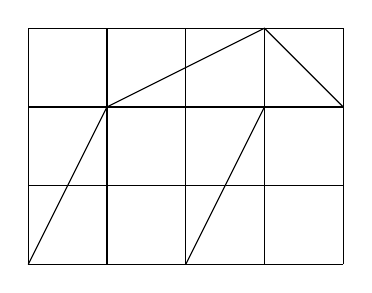
\begin{tikzpicture}
  \draw (0,0) grid(4,3);
  \draw (0,0) -- (1,2) -- (3,3) -- (4,2);
  \draw (2,0) -- (3,2);
\end{tikzpicture}
\vspace{.5cm}

% Example 3
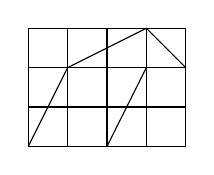
\begin{tikzpicture}[scale=.5]
  \draw (0,0) grid(4,3);
  \draw (0,0) -- (1,2) -- (3,3) -- (4,2);
  \draw (2,0) -- (3,2);
\end{tikzpicture}
\end{tcolorbox}
\end{minipage}
\end{tabularx}
\vspace{0.1cm}

There are also a number of options that can be passed to the \texttt{draw} command modifying the:

\noindent \textbf{Path Endpoints}

\vspace{.2cm}
\noindent
\begin{tabularx}{\textwidth}{@{}X p{0.4\textwidth}@{}}
\rowcolor{gray!30}
\textbf{\LaTeX{}} & \textbf{Formatted Output} \\

% LEFT: CODE INPUT
\begin{minipage}[t]{\linewidth}\vspace{0pt}
\footnotesize
\texttt{%
\% Line endpoints example \\
\textbackslash begin\{tikzpicture\} \\
\ \ \ \textbackslash draw [->] (0,2) $--$ (1,3); \\
\ \ \ \textbackslash draw [<-] (1,2) $--$ (2,3); \\
\ \ \ \textbackslash draw [|->] (2,2) $--$ (3,3); \\
\ \ \ \textbackslash draw [<->] (3,2) $--$ (4,3); \\
\ \ \ \textbackslash draw [<->] (1,1) $--$ (1,0) -- (3,0); \\
\textbackslash end\{tikzpicture\}
}
\end{minipage}
&
% RIGHT: FORMATTED OUTPUT
\begin{minipage}[t]{\linewidth}\vspace{0pt}
\footnotesize
\begin{tcolorbox}[colback=white, boxrule=0.3pt, arc=1mm, sharp corners]
\centering
\begin{tikzpicture}
  \draw [->] (0,2) -- (1,3);
  \draw [<-] (1,2) -- (2,3);
  \draw [|->] (2,2) -- (3,3);
  \draw [<->] (3,2) -- (4,3);
  \draw [<->] (1,1) -- (1,0) -- (3,0);
\end{tikzpicture}
\end{tcolorbox}
\end{minipage}
\end{tabularx}
\vspace{.1cm}

\noindent \textbf{Path Color, Style, \& Weight}
\begin{table}[H]
\centering
\renewcommand{\arraystretch}{1.2}
\begin{tabular}{p{\linewidth}}
\rowcolor{gray!30}
\textbf{\LaTeX{} Input} \\

\begin{minipage}{\linewidth}
\footnotesize
\texttt{%
\textbackslash begin\{tikzpicture\} \\
\ \ \ \% Color, style, \& weight examples\\
\ \ \ \textbackslash draw [->, thin, red] (0,2) $--$ (1,3); \\
\ \ \ \textbackslash draw [<-, thick, red] (1,2) $--$ (2,3); \\
\ \ \ \textbackslash draw [|->, ultra thick, dashed] (2,2) $--$ (3,3); \\
\ \ \ \textbackslash draw [<->, line width=0.1cm, blue] (3,2) $--$ (4,3); \\
\ \ \ \textbackslash draw [<->, line width=0.5mm, cyan, dotted] (4,2) $--$ (5,3); \\
\textbackslash end\{tikzpicture\}
}
\end{minipage}
\\[0.5em]

\rowcolor{gray!30}
\textbf{Formatted Output} \\

\begin{minipage}{\linewidth}
\centering
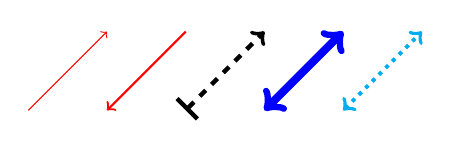
\begin{tikzpicture}
    \draw [->, thin, red] (0,2) -- (1,3);
    \draw [<-, thick, red] (1,2) -- (2,3);
    \draw [|->, ultra thick, dashed] (2,2) -- (3,3);
    \draw [<->, line width=0.1cm, blue] (3,2) -- (4,3);
    \draw [<->, line width=0.5mm, cyan, dotted] (4,2) -- (5,3);
\end{tikzpicture}
\end{minipage}
\end{tabular}
\end{table}

\subsection*{Drawing Shapes}
You are not limited to straight lines in TikZ. You can draw shapes like rectangles, circles, polygons and stars, etc. The following example depicts only a few.  You can also add the “rounded corners” option to lines and shapes to improve their appearance.

\begin{table}[H]
\centering
\renewcommand{\arraystretch}{1.2}
\begin{tabular}{p{\linewidth}}
\rowcolor{gray!30}
\textbf{\LaTeX{} Input} \\

\begin{minipage}{\linewidth}
\footnotesize
\texttt{%
\textbackslash begin\{tikzpicture\} \\
\ \ \ \textbackslash draw [blue, rounded corners] (0,0) rectangle (2,1); \\
\ \ \ \textbackslash draw [red, thick] (2,1) circle [radius=0.5]; \\
\ \ \ \textbackslash draw [green, ultra thick] (0,0.5) ellipse [x radius = 0.5cm, y radius = 1cm]; \\
\ \ \ \textbackslash draw [->, thick, dashed, rounded corners] (0,.5) $--$ (1,2) $--$ (2,1.5); \\
\textbackslash end\{tikzpicture\}
}
\end{minipage}
\\[0.5em]

\rowcolor{gray!30}
\textbf{Formatted Output} \\

\begin{minipage}{\linewidth}
\centering
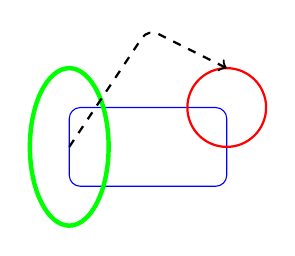
\begin{tikzpicture}
    \draw [blue, rounded corners] (0,0) rectangle (2,1);
    \draw [red, thick] (2,1) circle [radius=0.5];
    \draw [green, ultra thick] (0,0.5) ellipse [x radius = 0.5cm, y radius = 1cm];
    \draw [->, thick, dashed, rounded corners] (0,.5) -- (1,2) -- (2,1.5);
\end{tikzpicture}
\end{minipage}
\end{tabular}
\end{table}

You can also fill shapes and paths (when they are closed).  Notice the difference between the first two squares in the example below.  In the first red square, we indicated that the fill color should be red, but did not give a color for the \texttt{\textbackslash draw} line, so it is black. In the second red square, we indicated a color option that is also red, so the line produced by \texttt{\textbackslash draw} matches the fill color. 

\begin{table}[H]
\centering
\renewcommand{\arraystretch}{1.2}
\begin{tabular}{p{\linewidth}}
\rowcolor{gray!30}
\textbf{\LaTeX{} Input} \\

\begin{minipage}{\linewidth}
\footnotesize
\texttt{%
\textbackslash begin\{tikzpicture\} \\
\ \ \ \textbackslash draw [fill=red,ultra thick] (0,0) rectangle (1,1); \\
\ \ \ \textbackslash draw [fill=red,ultra thick,red] (2,0) rectangle (3,1); \\
\ \ \ \textbackslash draw [blue, fill=blue] (4,0) $--$ (5,1) $--$ (4.75,0.15) $--$ (4,0); \\
\ \ \ \textbackslash draw [fill] (7,0.5) circle [radius=0.1]; \\
\ \ \ \textbackslash draw [fill=orange] (9,0) rectangle (11,1); \\
\ \ \ \textbackslash draw [fill=white] (9.25,0.25) rectangle (10,1.5); \\
\textbackslash end\{tikzpicture\}
}
\end{minipage}
\\[0.5em]

\rowcolor{gray!30}
\textbf{Formatted Output} \\

\begin{minipage}{\linewidth}
\centering
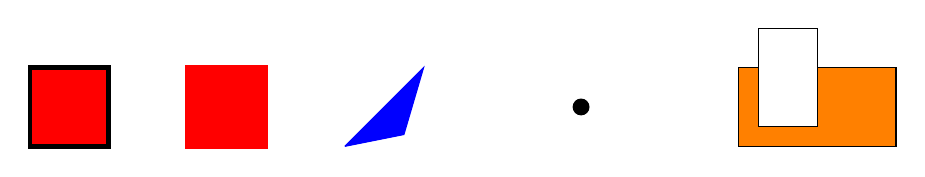
\begin{tikzpicture}
\draw [fill=red,ultra thick] (0,0) rectangle (1,1);
\draw [fill=red,ultra thick,red] (2,0) rectangle (3,1);
\draw [blue, fill=blue] (4,0) -- (5,1) -- (4.75,0.15) -- (4,0);
\draw [fill] (7,0.5) circle [radius=0.1];
\draw [fill=orange] (9,0) rectangle (11,1);
\draw [fill=white] (9.25,0.25) rectangle (10,1.5);
\end{tikzpicture}
\end{minipage}
\end{tabular}
\end{table}


\subsection*{Labeling Coordinates in a TikZ Picture}
When creating figures with TikZ, you often want to add labels or annotate parts of your drawing — for example, naming points, adding descriptions, or marking axes. This is easy to do with the \texttt{\textbackslash node} command. Think of \texttt{\textbackslash node} as a way to place text (or other content) at a specific coordinate or relative position inside your TikZ picture. Unlike \texttt{\textbackslash draw}, which creates lines and shapes, \texttt{\textbackslash node} creates a ``container'' for text or symbols (see examples below).

\vspace{.2cm}
\noindent
\begin{tabularx}{\textwidth}{@{}X p{0.25\textwidth}@{}}
\rowcolor{gray!30}
\textbf{\LaTeX{}} & \textbf{Formatted Output} \\

% Left cell: both LaTeX codes stacked
\begin{minipage}[t]{\linewidth}\vspace{0pt}
\footnotesize
\texttt{%
\textbackslash begin\{tikzpicture\} \\
\ \ \ \textbackslash draw [thick, <->] (0,2) $--$ (0,0) $--$ (2,0); \\
\ \ \ \textbackslash draw[fill] (1,1) circle [radius=0.025]; \\
\ \ \ \textbackslash node [below] at (1,1) \{below\}; \\
\ \ \ \textbackslash node [above] at (1,1) \{above\}; \\
\ \ \ \textbackslash node [left] at (1,1) \{left\}; \\
\ \ \ \textbackslash node [right] at (1,1) \{right\}; \\
\textbackslash end\{tikzpicture\} \\
\\[1em]
\textbackslash begin\{tikzpicture\}[xscale=3, yscale=1.5] \\
\ \ \ \textbackslash draw [thick, <->] (0,1) $--$ (0,0) $--$ (1,0); \\
\ \ \ \textbackslash node [below right] at (1,0) \{\$x\$\}; \\
\ \ \ \textbackslash node [above left] at (0,1) \{\$y\$\}; \\
\ \ \ \textbackslash draw [fill] (.4,.7) circle [radius=.5pt]; \\
\ \ \ \textbackslash node [above right, align=left] at (.4,.7) \{This is a point\}; \\
\ \ \ \textbackslash node [below, align=center] at (.5,0) \{A centered \textbackslash\textbackslash x-axis label\}; \\
\textbackslash end\{tikzpicture\}
}
\end{minipage}
&
% Right cell: both rendered outputs stacked
\begin{minipage}[t]{.7\linewidth}\vspace{0pt}
\centering
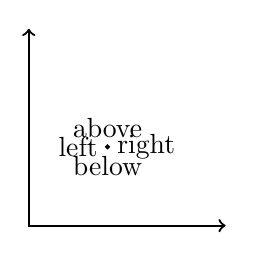
\begin{tikzpicture}
\draw [thick, <->] (0,2.5) -- (0,0) -- (2.5,0);
\draw[fill] (1,1) circle [radius=0.025];
\node [below] at (1,1) {below};
\node [above] at (1,1) {above};
\node [left] at (1,1) {left};
\node [right] at (1,1) {right};
\end{tikzpicture}

\vspace{3em}

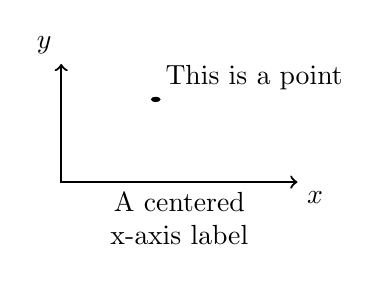
\begin{tikzpicture}[xscale=3, yscale=1.5]
\draw [thick, <->] (0,1) -- (0,0) -- (1,0);
\node [below right] at (1,0) {$x$};
\node [above left] at (0,1) {$y$};
\draw [fill] (.4,.7) circle [radius=.5pt];
\node [above right, align=left] at (.4,.7) {This is a point};
\node [below, align=center] at (.5,0) {A centered \\ x-axis label};
\end{tikzpicture}
\end{minipage}
\end{tabularx}

\subsection*{Path Diagrams}
Path diagrams are frequently used in the Psychological Sciences to represent relationships between variables (e.g., correlation, mediation, moderation), and to illustrate statistical models and theoretical frameworks. When creating path diagrams, using LaTeX with TikZ offers several advantages over point-and-click software like PowerPoint. TikZ produces vector-based graphics that integrate seamlessly into your LaTeX document, ensuring consistent fonts, mathematical notation, and styles throughout your work without the need to manually match formatting. Unlike PowerPoint, where precise positioning can be tedious and prone to misalignment, TikZ allows you to define elements and their relationships using exact coordinates or relative positioning commands, guaranteeing reproducibility and pixel-perfect accuracy. This approach is especially valuable for academic work, where diagrams often need to be updated, scaled, or reused — with TikZ, you can modify a few lines of code rather than rebuilding the figure from scratch. Furthermore, because TikZ diagrams are text-based, they are version-control-friendly, enabling collaboration and easy tracking of changes. In short, LaTeX+TikZ combines precision, scalability, and reproducibility in a way that point-and-click tools cannot match, making it the preferred choice for professional, publication-quality path diagrams.

In TikZ, the \texttt{\textbackslash path} command is the most general way to describe a sequence of points, curves, and shapes — but by itself, it doesn't actually produce any visible output. Think of \texttt{\textbackslash path}  as defining a route or shape, but \LaTeX has not yet been told what to do with it.…however, when \texttt{\textbackslash path} is combined with the \texttt{draw} argument or provided a color argument, its behavior is similar to the \texttt{\textbackslash draw} command. \texttt{\textbackslash path} is sometimes preferred because it is more general: it can define complex geometric paths without immediately rendering them, allowing those paths to be reused, transformed, or drawn/fill-stroked later in different ways. This separation of path definition from path rendering can make code more modular, easier to maintain, and better suited for situations where the same geometry needs to be styled multiple times.

The example below illustrates how nodes and paths can be combined to produce flexible diagrams in your \LaTeX document.

\begin{table}[H]
\centering
\renewcommand{\arraystretch}{1.2}
\begin{tabular}{p{\linewidth}}
\rowcolor{gray!30}
\textbf{\LaTeX{} Input} \\

\begin{minipage}{\linewidth}
\footnotesize
\texttt{%
\textbackslash begin\{tikzpicture\} \\
\ \ \ \textbackslash node[align=right](1)at(0,0)\{Bad\textbackslash \textbackslash Parenting\}; \\
\ \ \ \textbackslash node[blue,align=center](2)[right=of 1]\{Risk\textbackslash \textbackslash Taking\};\\
\ \ \ \textbackslash node[align=left](3)[right=of 2]\{Premature\textbackslash \textbackslash Death\}; \\
\ \ \ \textbackslash node[red](4)[below=of 2]\{Depression\};\\
\ \ \ \textbackslash path[->](1)edge(2); \\
\ \ \ \textbackslash path[blue](2)edge(3);\\
\ \ \ \textbackslash path[red,line width=.8mm](4)edge(3);\\
\ \ \ \textbackslash path(1)edge(4);\\
\textbackslash end\{tikzpicture\}
}
\end{minipage}
\\[0.5em]

\rowcolor{gray!30}
\textbf{Formatted Output} \\

\begin{minipage}{\linewidth}
\centering
\begin{tikzpicture}
    \node[align=right](1)at(0,0){Bad\\ Parenting};
    \node[blue,align=center](2)[right=of 1]{Risk\\Taking};
    \node[align=left](3)[right=of 2]{Premature\\Death};
    \node[red](4)[below=of 2]{Depression};
    \path[->](1)edge(2);
    \path[blue](2)edge(3);
    \path[red,line width=.8mm](4)edge(3);
    \path(1)edge(4);
\end{tikzpicture}

\end{minipage}
\end{tabular}
\end{table}


You may have noticed that there are many different options that can be passed to the \texttt{\textbackslash node} and \texttt{\textbackslash path} commands.  Rather than explain them all, let's just consider the TikZ command below:

\begin{verbatim}
\node [blue, align=center](2)[right=of 1]{Risk\\Taking};
\end{verbatim}

\noindent This command places a labeled node in a TikZ picture. Let's break down each part:

\begin{description}
  \item[\textbf{\texttt{\textbackslash node}}] This is the basic command used to create a node, which is a point in the graphic that can contain text or shapes.
  
  \item[\textbf{\texttt{[blue,align=center]}}] The first optional argument specifies styling options, in this case:
  \begin{itemize}
    \item \texttt{blue} — sets the color of the text (and the node border if drawn) to blue.
    \item \texttt{align=center} — centers multi-line text inside the node.
  \end{itemize}
  
  \item[\textbf{\texttt{(2)}}] This assigns the \emph{name} \texttt{``2''} to the node, which allows referencing this node later when drawing edges or positioning other nodes.
  
  \item[\textbf{\texttt{[right=of 1]}}] The second optional argument (another set of brackets) is a positioning directive:
  \begin{itemize}
    \item \texttt{right=of 1} — places this node to the right of the node named \texttt{1}. 
    \item Note that this requires the \texttt{positioning} library, loaded with \texttt{\textbackslash usetikzlibrary\{positioning\}} in the preamble.
  \end{itemize}

  \item[\textbf{\texttt{\{Risk\textbackslash \textbackslash Taking\}}}] This is the node content enclosed in curly braces:
  \begin{itemize}
    \item \texttt{Risk\textbackslash \textbackslash Taking} — the double backslash \texttt{\\} creates a line break, so the text is displayed on two centered lines.
  \end{itemize}
\end{description}

\bigskip
\noindent
In summary, when used inside a \texttt{tikzpicture} environment (with a node named \texttt{1} defined), this will create a blue-colored, two-line label positioned directly to the right of the node named \texttt{1}.

In practice of course, it is usually the case that nodes and arrows will all have the same (or similar) formatting.  Below is and example of a simple path diagram illustrating the prediction that both risk taking and depression may be mediators of the relationship between bad parenting and an increased likelihood of premature death.

\begin{table}[H]
\centering
\renewcommand{\arraystretch}{1.2}
\begin{tabular}{p{\linewidth}}
\rowcolor{gray!30}
\textbf{\LaTeX{} Input} \\

\begin{minipage}{\linewidth}
\footnotesize
\texttt{%
\textbackslash begin\{tikzpicture\} \\
   \ \ \ \textbackslash node[draw, align=center, minimum width=0.7cm, inner sep=2pt](1) at (0,0) {Bad\textbackslash \textbackslash Parenting};\\
   \ \ \ \textbackslash node[draw, align=center, minimum width=0.7cm, inner sep=2pt](2)[right=of 1]{Risk\textbackslash \textbackslash Taking};\\
   \ \ \ \textbackslash node[draw, align=center, minimum width=0.7cm, inner sep=2pt](3)[right=of 2]{Premature\textbackslash \textbackslash Death};\\
  \ \ \ \textbackslash node[draw, align=center, minimum width=0.7cm, inner sep=2pt](4)[below=of 2]{Depression};\\
    \ \ \ \textbackslash path[->,thick](1)edge(2);\\
    \ \ \ \textbackslash path[->,thick](2)edge(3);\\
    \ \ \ \textbackslash path[->,thick](4)edge(3);\\
    \ \ \ \textbackslash path[->,thick](1)edge(4);\\
\textbackslash end\{tikzpicture\}
}
\end{minipage}
\\[0.5em]

\rowcolor{gray!30}
\textbf{Formatted Output} \\

\begin{minipage}{\linewidth}
\centering
\begin{tikzpicture}
   \node[draw, align=center, minimum width=0.7cm, inner sep=2pt](1) at (0,0) {Bad\\ Parenting};
   \node[draw, align=center, minimum width=0.7cm, inner sep=2pt](2)[right=of 1]{Risk\\Taking};
   \node[draw, align=center, minimum width=0.7cm, inner sep=2pt](3)[right=of 2]{Premature\\Death};
   \node[draw, align=center, minimum width=0.7cm, inner sep=2pt](4)[below=of 2]{Depression};
    \path[->,thick](1)edge(2);
    \path[->,thick](2)edge(3);
    \path[->,thick](4)edge(3);
    \path[->,thick](1)edge(4);
\end{tikzpicture}

\end{minipage}
\end{tabular}
\end{table}

Again, a major advantage of using TikZ in this context is the precision with which elements can be controlled.  For example, the text of each box is perfectly equally padded with space within the box and all lines leading from/to the boxes attach at exactly the same points (predetermined by TikZ), and we have only scratched the surface!  Below is a more complex example that adds model estimates from the regression and some curved lines.


\begin{table}[H]
\centering
\renewcommand{\arraystretch}{1.2}
\begin{tabular}{p{\linewidth}}
\rowcolor{gray!30}
\textbf{\LaTeX{} Input} \\

\begin{minipage}{\linewidth}
\scriptsize
\texttt{%
\textbackslash begin\{tikzpicture\} \\
   \ \ \ \textbackslash node [draw, align=center, minimum width=2cm, minimum height=2cm, inner sep=2pt] (1) at(0,0){Bad\textbackslash \textbackslash Parenting};\\
   \ \ \ \textbackslash node [draw, align=center, minimum width=2cm, minimum height=2cm, inner sep=2pt] (2) [right=of 1] \{Risk\textbackslash \textbackslash Taking\};\\
   \ \ \ \textbackslash node [draw, align=center, minimum width=2cm, minimum height=2cm, inner sep=2pt] (3) [right=of 2]\{Premature\textbackslash \textbackslash Death\};\\
   \ \ \ \textbackslash node [draw, align=center, minimum width=2cm, minimum height=2cm, inner sep=2pt] (4) [below=of 2]\{Depression\};\\
   \ \ \ \textbackslash path[->,thick](1)edge(2);\\
   \ \ \ \textbackslash path[->,thick](2)edge(3);\\
   \ \ \ \textbackslash path[->,thick](4.east)edge(3.west);\\
   \ \ \ \textbackslash path[->,thick](1.east)edge node[pos=0.5, left=1pt] \{0.2\}(4.west);\\
   \ \ \ \textbackslash path[<->,thick,dashed](1.north)edge[bend left=30] node[above] \{\$\textbackslash beta=0.5\$\}(3.north);\\
\textbackslash end\{tikzpicture\}
}
\end{minipage}
\\[0.5em]

\rowcolor{gray!30}
\textbf{Formatted Output} \\

\begin{minipage}{\linewidth}
\centering
\begin{tikzpicture}
    \node [draw, align=center, minimum width=2cm, minimum height=2cm, inner sep=2pt] (1) at(0,0){Bad\\Parenting};
    \node [draw, align=center, minimum width=2cm, minimum height=2cm, inner sep=2pt] (2) [right=of 1] {Risk\\Taking};
    \node [draw, align=center, minimum width=2cm, minimum height=2cm, inner sep=2pt] (3) [right=of 2]{Premature\\Death};
    \node [draw, align=center, minimum width=2cm, minimum height=2cm, inner sep=2pt] (4) [below=of 2]{Depression};
    \path[->,thick](1)edge(2);
    \path[->,thick](2)edge(3);
    \path[->,thick](4.east)edge(3.west);
    \path[->,thick](1.east)edge node[pos=0.5, left=1pt] {0.2}(4.west);
    \path[<->,thick,dashed](1.north)edge[bend left=30] node[above] {$\beta=0.5$}(3.north);
\end{tikzpicture}

\end{minipage}
\end{tabular}
\end{table}

There are a few things to note about the example above:
\begin{itemize}
\item The \texttt{minimum width} and \texttt{minimum height} arguments were used to make the box size constant across nodes.
\item Two of the paths include the \texttt{node} command that is used to add text to a path.  Note that the \texttt{node} command also takes arguments used to position the text appropriately. 
\item The math environment (e.g., \$...\$) can be used to insert equations or Greek letters along paths.
\end{itemize}

\subsection*{Experimental Design Layouts and Task Schematics (UNDER CONSTRUCTION)}
Experimental design layouts are crucial diagrams in psychological science for visually organizing and representing the structure of experiments, including factors, conditions, and participant groups. These layouts help clarify complex designs such as within-subjects, between-subjects, or mixed factorial experiments by depicting how participants experience different conditions and how variables are manipulated. By mapping these elements graphically, researchers can better plan studies, communicate methodology, and understand interactions among factors. TikZ allows precise control over node placement and connections to illustrate experimental setups clearly and professionally.

\subsubsection{Experimental Design Layouts}


\subsection*{Putting it All Together}
	The previous sections introduce all of the commands needed to create an entire \LaTeX document in APA style.  For those new to markup languages like \LaTeX, creating your first complete document can seem like a daunting task.  One way to simplify the process is to organize each section of the document into separate files.  For example, many \LaTeX users will place the \texttt{documentclass} command and the preamble into a file called \texttt{main.tex}.  The introduction, method, results, and discussion would each be contained in separate \texttt{.tex} files an included in the \texttt{main} document using the \texttt{\textbackslash include\{doc.tex\}} command.  Visit \weblink{https://www.overleaf.com/read/sdyytvnmjfst} in any browser to see a complete example of a \LaTeX manuscript following the APA 7th edition style.

\section{Tips \& Tricks}
\subsection*{Placing Figures Inline with Text}
Before the release of the APA 7th edition guidelines, tables and figures were expected to appear at the end of the document, each on their own page. This remains the default behavior of the apa7 document class. However, APA 7 also allows authors to place figures and tables inline with the text, on the same page where they are first mentioned. This is often preferable when you want the reader to immediately see the figure or table without flipping pages.

To override the default behavior, add the \texttt{floatsintext} option to your \texttt{\textbackslash documentclass} line. For example:

\begin{center}
\texttt{\textbackslash documentclass[a4paper,man,natbib,floatsintext]\{apa7\}}
\end{center}

Once this is done, you can place your figure or table environments exactly where you want in the flow of the text, and LaTeX will try to keep them close to where they are introduced.

By default, LaTeX tries to keep the caption with the corresponding figure or table, but if there’s a page break issue or a lot of surrounding text, they can sometimes get separated or placed awkwardly. To force them to stick together:

Always put the \texttt{\textbackslash caption\{...\}} inside the float environment (figure or table). For example, using:
\begin{verbatim}
\begin{figure}[htbp]
  \centering
  \includegraphics[width=0.7\textwidth]{myfigure}
  \caption{An example figure that will always keep its caption.}
  \label{fig:example}
\end{figure}
\end{verbatim}
\noindent will prevent page breaks between caption and table/figure description

Another option is to add \texttt{\textbackslash usepackage\{caption\}} to the preamble and use the skip option to control spacing, which also helps keep things tight:

\begin{verbatim}
\usepackage[skip=5pt]{caption}
\end{verbatim}

If \LaTeX still tries to split up the elements of a figure or table, wrap the float in a minipage to lock the figure/table and caption into one unbreakable unit:
\begin{verbatim}
\begin{figure}[H] % requires \usepackage{float}
  \begin{minipage}{\linewidth}
    \centering
    \includegraphics[width=0.7\textwidth]{myfigure}
    \caption{Caption that will never be separated from the figure.}
    \label{fig:example}
  \end{minipage}
\end{figure}
\end{verbatim}

\noindent For tables specifically:
If your table has a description below it (common in APA), include the description inside the float as normal text after the \texttt{\textbackslash caption\{...\}}. This way \LaTeX considers the whole thing one object.

\begin{verbatim}
\begin{table}[htbp]
  \centering
  \caption{Participant demographics}
  \begin{tabular}{ll}
    \hline
    Age & Mean (SD) \\
    \hline
    25 & (3.2) \\
    \hline
  \end{tabular}
  \vspace{2mm}
  \footnotesize\textit{Note.} Data represent means and standard deviations.
\end{table}
\end{verbatim}

\section{Additional Resources}
An advantage of \LaTeX is that it has been around for a long time and has a huge, global user base.  That means that most questions you have can be answered using any internet search engine.  In fact I recommend using the internet as much as possible when you encounter questions and/or problems.  However, if you are looking for some additional readings/references, below is a short list of some good resources:
\begin{itemize}
\item \LaTeX on Wikibooks: \weblink{https://en.wikibooks.org/wiki/LaTeX}

\item The Not So Short Introduction to \LaTeX 2E by Tobias Oetiker, Hubert Partl, Irene Hyna, and Elisabeth Schlegl: \weblink{https://archive.org/details/lshort}

\item Guide to \LaTeX (4th edition) by Helmut Kopka and Patrick W. Daly: \weblink{http://www.worldcat. org/oclc/844889428}

\item Overleaf \LaTeX Tips: \weblink{https://www.overleaf.com/help/category/latex_tips}
\item Overleaf Video Tutorials: \weblink{https://www.overleaf.com/help/category/video_tutorials} 
\end{itemize}


\newpage
\section{Assignment}
\subsubsection{Overview}
In this assignment, you will learn to create a professionally formatted psychological research report using LaTeX, focusing on the formatting guidelines of the American Psychological Association (APA) 7th edition. Learning to use LaTeX for your research reports not only enhances your technical skills but also helps you produce clean, consistent, and reproducible documents that are widely valued in the academic community.

\subsubsection{Instructions}
To complete this assignment, you will use the APA template in the \texttt{Latex\_and\_Git} directory of your personal branch of the forked GitHub repository found at \weblink{https://github.com/pdkieffaber/PSYC672}.  In order to get credit for this assignment, you should:
\begin{enumerate}
\item Modify the document preamble (main.tex) to be consistent with your project.
\item Modify the Introduction section (intro.tex) to include a brief 1-2 page background related to your current or anticipated project that includes at least two references to relevant published work.  The introduction should include a clear statement of the primary hypothesis and end with a brief description of how that hypothesis will be addressed in the current study.
\item Modify the Method section (method.tex) to fit with your research methods.  Bullet points are fine.
\item Modify the Results section (results.tex) to fit with your data analysis.  Bullet points are fine.
\item Modify the Discussion section (discussion.tex) to fit with your results (actual or expected).  Just a couple sentences about how your research will contribute to the broader literature is fine.
\item Push your modifications to your personal branch of the PSYC672 GitHub repo.
\end{enumerate}


\printglossary[type=intro2latex,style=twocolumn]
%\printglossary
%\glsresetall
\newpage
\bibliographystyle{apalike}
\renewcommand{\bibname}{References}
\bibliography{bibliography}
